\chapter{Verifying Topology of Isosurface Extraction Algorithms}\label{chap:topology}

Visualization is an important aspect of current large-scale
data analysis.
%
As the users of scientific software are not typically visualization
experts,
%
they might not be aware of limitations
and properties of the underlying algorithms and visualization
techniques.
%
As visualization researchers and practitioners, it is our responsibility to
ensure that these limitations and properties are clearly stated and studied.
%
Moreover, we should provide mechanisms which attest to the correctness of 
visualization systems.
%
Unfortunately, the accuracy, reliability, and robustness of visualization
algorithms and their implementations have not in general fallen under
such scrutiny as have other components of the scientific computing
pipeline.
%

%The main goal of verifiable visualization is to increase confidence in
%visualization tools~\cite{kirby-vv-08}.
%%,and is the main motivation of this paper as well.  
%Verifiable visualization tries to develop systematic mechanisms for
%identifying and correcting errors in both algorithms and
%implementations of visualization techniques.  As an example, consider
%a recent scheme to check geometrical properties of isosurface
%extraction~\cite{etiene:tvcg:2009}.  By writing down easily checkable
%convergence properties that the programs should exhibit, the authors
%identified bugs in isosurfacing codes that had gone undetected.

We strive for verification tools which are both \emph{simple} and
\emph{effective}. Simple verification methods are less likely to have
bugs themselves, and effective methods make it difficult for bugs to
hide.  Alas, the mathematical properties of an algorithm and its
implementation are both constructs of fallible human beings, and so
perfection is an unattainable goal; there will always be the next
bug. Verification is, fundamentally, a \emph{process}, and when it
finds problems with an algorithm or its implementation, we can only
claim that the new implementation behaves more correctly than the old
one.  Nevertheless, the verification process clarifies \emph{how} the
implementations fail or succeed.

In this chapter, we investigate isosurfacing algorithms and
implementations and focus on their \emph{topological properties}. For
brevity, we will use the general phrase ``isosurfacing'' when we refer
to both isosurfacing algorithms and their implementations.
%
As a simple example, the topology of the output of isosurface codes
should match that of the level set of the scalar field (as discussed
in Section \ref{sec:problem}).
%
Broadly speaking, we use the method of manufactured solutions (MMS) to
check these properties.
%
By manufacturing a model whose known behavior should be reproduced by
the techniques under analysis, MMS can check whether they meet
expectations.

%Etiene \emph{et al.} have recently used this method to verify geometrical properties of
%isosurfacing codes~\cite{etiene:tvcg:2009}, and topological
%verification naturally follows.
%
An important contribution of this work is the selection of
significant topological characteristics that can be verified by
software methods.
%
We use results from two fields in computational topology, namely
digital topology and stratified Morse theory.
%
% The
% selection of compelling test cases requires not only conceptual insight, but also
% experimental testing.

In summary, the main contributions of this work can be stated as
follows:
\begin{enumerate}
\item In the spirit of verifiable visualization, we introduce a
  methodology for checking topological properties of publicly and
  commercially available isosurfacing software.
\item We show how to adapt techniques from digital topology to yield simple
  and effective verification tools for isosurfaces without
  boundaries.
\item We introduce a simple technique to compute the Euler
  characteristic of a level set of a trilinearly interpolated scalar
  field. The technique relies on stratified Morse theory and allows
  us to verify topological properties of isosurfaces with boundaries.
\item We propose a mechanism to manufacture isosurfaces with
  non-trivial topological properties, showing that this simple
  mechanism effectively stresses isosurfacing programs. As input, we
  also assume a piecewise trilinear scalar field defined on a regular
  grid.
% cscheid: The sentence below does not belong here.
%
% We should clarify that when applying MMS for other techniques (and even in
% the case of isosurface extraction), the theoretical analysis should be
% tailored to the particular features of these algorithms.
%
%as the same framework 
%can be adopted to scrutinizing other visualization methods.
\end{enumerate}
The verification process produces a comprehensive record of the desired properties
of the implementations, along with an objective assessment of whether these
properties are satisfied. This record improves the
applicability of the technique and increases the value of
visualization.
%
%% Finally, we stress that a valuable by-product of the verification process is
%% a comprehensive record of the desired properties of the results of the
%% technique, along with an objective assessment of whether or not
%% these properties are satisfied.
%
%% This record improves
%% the applicability of the technique under verification and increases 
%% the value of the contributions of visualization for the computational science community.
%
We present a set of results obtained using our method, and we report
errors in two publicly-available isosurface extraction codes.
%which claim topological properties.

\section{Related Work}
\label{sec:rw}
 
The literature that evaluates isosurface extraction
techniques is enormous, with works ranging from mesh
quality~\cite{Dietrich:TVCG:2008,Schreiner06,Raman:2008:QIM}, to
performance~\cite{Sutton00acase} and accuracy
analysis~\cite{patera04,zhou01}.
%
In this section, we focus
on methods that deal with
topological issues that naturally appear in isosurfacing. 

%\paragraph*{Topology-aware Isosurfacing}
\textbf{Topology-aware Isosurfacing}.
Arguably the most popular isosurface extraction technique, Marching Cubes~\cite{lor87}
(MC) processes one grid cell 
at a time and uses the \emph{signs} of each grid node (whether
the scalar field at the node is above or below the isovalue) to fit a triangular mesh that
approximates the isosurface within the cell.
As no information besides the signs is taken into account, Marching
Cubes cannot guarantee any topological 
equivalence between the triangulated mesh and the original isosurface. In fact,
the original Marching
Cubes algorithm would produce surfaces with
``cracks,'' caused by alternating vertex signs along a face boundary,
which lead to contradicting triangulations in neighboring cells~\cite{Nielson:1991:ADR:949607.949621}.
Disambiguation mechanisms can ensure crack-free surfaces,
and many schemes have been proposed, such as
the one by Montani \emph{et al.}~\cite{Montani:1994:MLT},
domain tetrahedralization~\cite{Hamish06}, 
preferred polarity~\cite{Bloomenthal88}, gradient-based method~\cite{gelder:tog:1994}, and
feature-based schemes~\cite{ho:cgf:2005}.
%
The survey of Newman and Yi has a comprehensive account~\cite{newman:candg:2006}.
%
Although disambiguation prevents cracks in the output, it does not
guarantee topological equivalence.

Topological equivalence between the resulting triangle mesh and the isosurface
can only be achieved with additional information about the underlying
scalar field.
%
Since function values on grid nodes are typically the only information
provided, a reconstruction kernel is assumed, of which trilinear
reconstruction on regular hexahedral grids is most
popular~\cite{Nielson03onmarching}.
%
Nielson and
Hamann, for example,
use saddle points of the bilinear
interpolant on grid cell faces~\cite{Nielson:1991:ADR:949607.949621}. 
%
Their method cannot always reproduce the
topology of trilinear interpolation because there remain  ambiguities
internal to a grid cell: pairs of non-homeomorphic isosurfaces could
be homeomorphic when restricted to the grid cell faces.
%
This problem has been recognized by Natarajan~\cite{Natarajan:1994:GTC:205424.205429} and 
Chernyaev~\cite{Chernyaev95marchingcubes}, leading to new classification and
triangulation schemes.
%
This line of work has inspired many other ``topology-aware'' triangulation
methods,
such as Cignoni \emph{et al.}'s reconstruction
technique~\cite{Cignoni00reconstructionof}.
%
Subsequent work by Lopes and Brodlie~\cite{lopes:tvcg:2003} and
Lewiner \emph{et al.}~\cite{Lewiner:2003} has finally provided triangulation patterns covering
all possible topological configurations of trilinear functions, implicitly promising
a crack-free surface.
%
The topology of the level sets generated by trilinear interpolation
has been recently studied by Carr and Snoeyink~\cite{CS08}, and Carr
and Max~\cite{10.1109/TVCG.2009.10}. A discussion about these can be found in
Section~\ref{sec:smt}.

% \paragraph*{Verifiable Visualization}
\textbf{Verifiable Visualization}.
Many of the false steps in the route from the
original MC algorithm to the recent homeomorphic solutions
could have been avoided with a systematic procedure to verify the
algorithms and the corresponding implementations. 
%
Although the lack of verification of visualization techniques and the
corresponding software implementations has been a long-term concern of
the visualization community~\cite{globus95,kirby-vv-08}, concrete
proposals on verification are relatively recent.
%
Etiene \emph{et al.}~\cite{etiene:tvcg:2009} were among the first
in scientific visualization to propose a practical
verification framework for geometrical properties of isosurfacing.
Their work is
based on the method of manufactured solutions (MMS),
a popular approach for assessing numerical software~\cite{babuska04}. 
We are interested in \emph{topological properties} of
isosurfacing, and we also use MMS as a
verification mechanism. As we will show in Section~\ref{sec:results}, our proposed
technique discovered problems in popular software,
supporting our assertion about the value of a
broader culture of verification in scientific visualization.

There have been significant theoretical investigations in computational
topology dealing with, for example, isosurface invariants, persistence, and stability~
\cite{Cohen-Steiner07, edelsbrunner10}.
%
This body of work is concerned with how to
define and compute topological properties of computational objects. 
%
We instead develop methods that stress topological properties of isosurfacing.
%
These goals are complementary.
%
Computational topology 
tools for data analysis might offer new properties which can be used
for verification purposes, and verification tools can
assess the correctness of the computational topology implementations.
%
Although the mechanism we propose to compute topological invariants
for piecewise smooth scalar fields is, to the best of our knowledge,
novel (see Section~\ref{sec:smt}), our primary goal is to present a
method that developers can adapt to assess their own software.

%There has been significant theoretical investigations in the field of
%computational topology, where algorithm correctness is a major concern and
%indeed carefully proven \cite{Cohen-Steiner07, edelsbrunner10}  (computation of the topological invariants of
%isosurfaces, persistence simplification of topological spaces, stability of of
%geometrical measures). However, most of these works study the piecewise linear
%setting (triangulations), which benefits from many nice combinatorial
%properties leading to sound correctness assessments. In contrast, due to their
%more application-oriented concerns, visualization techniques have been mostly
%built around data-representations involving more complex interpolants (like
%the trilinear), where more ambiguity naturally arises. Moreover, to the best
%of our knowledge, no methodology has been proposed in the computational
%topology community toward stressing isosurfacing codes in order to verify
%their topological correctness.

\section{Verifying Isosurface Topology}
\label{sec:problem}

We now discuss strategies for verifying topological
properties of isosurfacing techniques. 
%
We start by observing that simply stating the desired properties of
the implementation is valuable.
%
Consider a typical implementation of Marching Cubes.
%
How would you debug it?
%
Without a small set of desired properties, we are mostly limited to
inspecting the output by explicitly exercising every case in the case
table. The fifteen cases might not seem daunting, but what if we
suspect a bug in symmetry reduction? We now have 256 cases
to check. Even worse, what if the bug is in a combination of separate
cases along neighboring cells?
%
The verification would grow to be at least as complicated as the
original algorithm, and we would just as likely make a mistake during
the verification as we would in the implementation.
%
Therefore, we need properties that are simple to state, easy to check,
and good at catching bugs.

\textbf{Simple example}. Although the previously mentioned problem
with Marching Cubes~\cite{lor87} is well-known, it is not
immediately clear what topological properties
fail to hold. For example, ``the output of Marching Cubes cannot
contain boundary curves'' is not one such property, for two
reasons. First, some valid surfaces generated by Marching Cubes --
such as with the simple $2^3$ case -- do contain boundaries. Second,
many incorrect outputs might not contain any boundaries at all. The
following might appear to be a good candidate property: ``given a
positive vertex $v_0$ and a negative vertex $v_1$, any path through
the scalar field should intersect the isosurface an odd number of
times.'' This property \emph{does} capture the fact that the triangle
mesh should separate interior vertices from exterior vertices and
seems to isolate the problem with the cracks. Checking this property,
on the other hand, and even stating it precisely, is
problematic. Geometrical algorithms for intersection tests are
notoriously brittle; for example, some paths might intersect the
isosurface in degenerate ways.  A more promising approach comes from
noticing that any such separating isosurface has to be a piecewise-linear
manifold, whose boundary must be a subset of the boundary of the
grid. This directly suggests that ``the output of Marching Cubes must
be a piecewise-linear (PL) manifold whose boundaries are contained in
the boundary of the grid.''  This property is simple to state and easy
to test: the link of every interior vertex in a PL manifold is
topologically a circle, and the link of every boundary vertex is a
line.
%
The term ``consistency'' has been used to describe problems with some
algorithms~\cite{newman:candg:2006}. In this work, we say that the
output of an algorithm is \emph{consistent} if it obeys the PL
manifold property above.  By generating arbitrary grids and extracting
isosurfaces with arbitrary isovalues, the inconsistency of the
original case table becomes mechanically checkable and instantly
apparent.
%
Some modifications to the basic Marching Cubes table, such as using
Nielson and Hamann's asymptotic decider~\cite{Nielson:1991:ADR:949607.949621}, result in
consistent implementations, and the outputs pass the PL manifold
checks (as we will show in Section~\ref{sec:results}).

The example we have presented above is a complete instance of the
method of manufactured solutions. We identify a property that the
results should obey, run the implementations on inputs, and test
whether the resulting outputs respect the properties.
%
In the next sections, we develop a verification method for algorithms
to reproduce the topology of the level sets of trilinear
interpolation~\cite{Chernyaev95marchingcubes,lopes:tvcg:2003,Nielson03onmarching},
thus completely eliminating any ambiguity. In this work, we say the
output is \emph{correct} if it is homeomorphic to the corresponding
level set of the scalar field.
%
This correctness property is simple to state, but developing effective
verification schemes that are powerful and simple to implement is more
involved. We will turn to invariants of topological spaces, in
particular to Betti numbers and the Euler characteristic, 
their relative strengths and weaknesses, and discuss how to robustly check
their values.  Figure~\ref{fig:pipeline} shows our pipeline to assess
topological correctness and also the chapter organization.

\begin{figure}[b]
\begin{center}
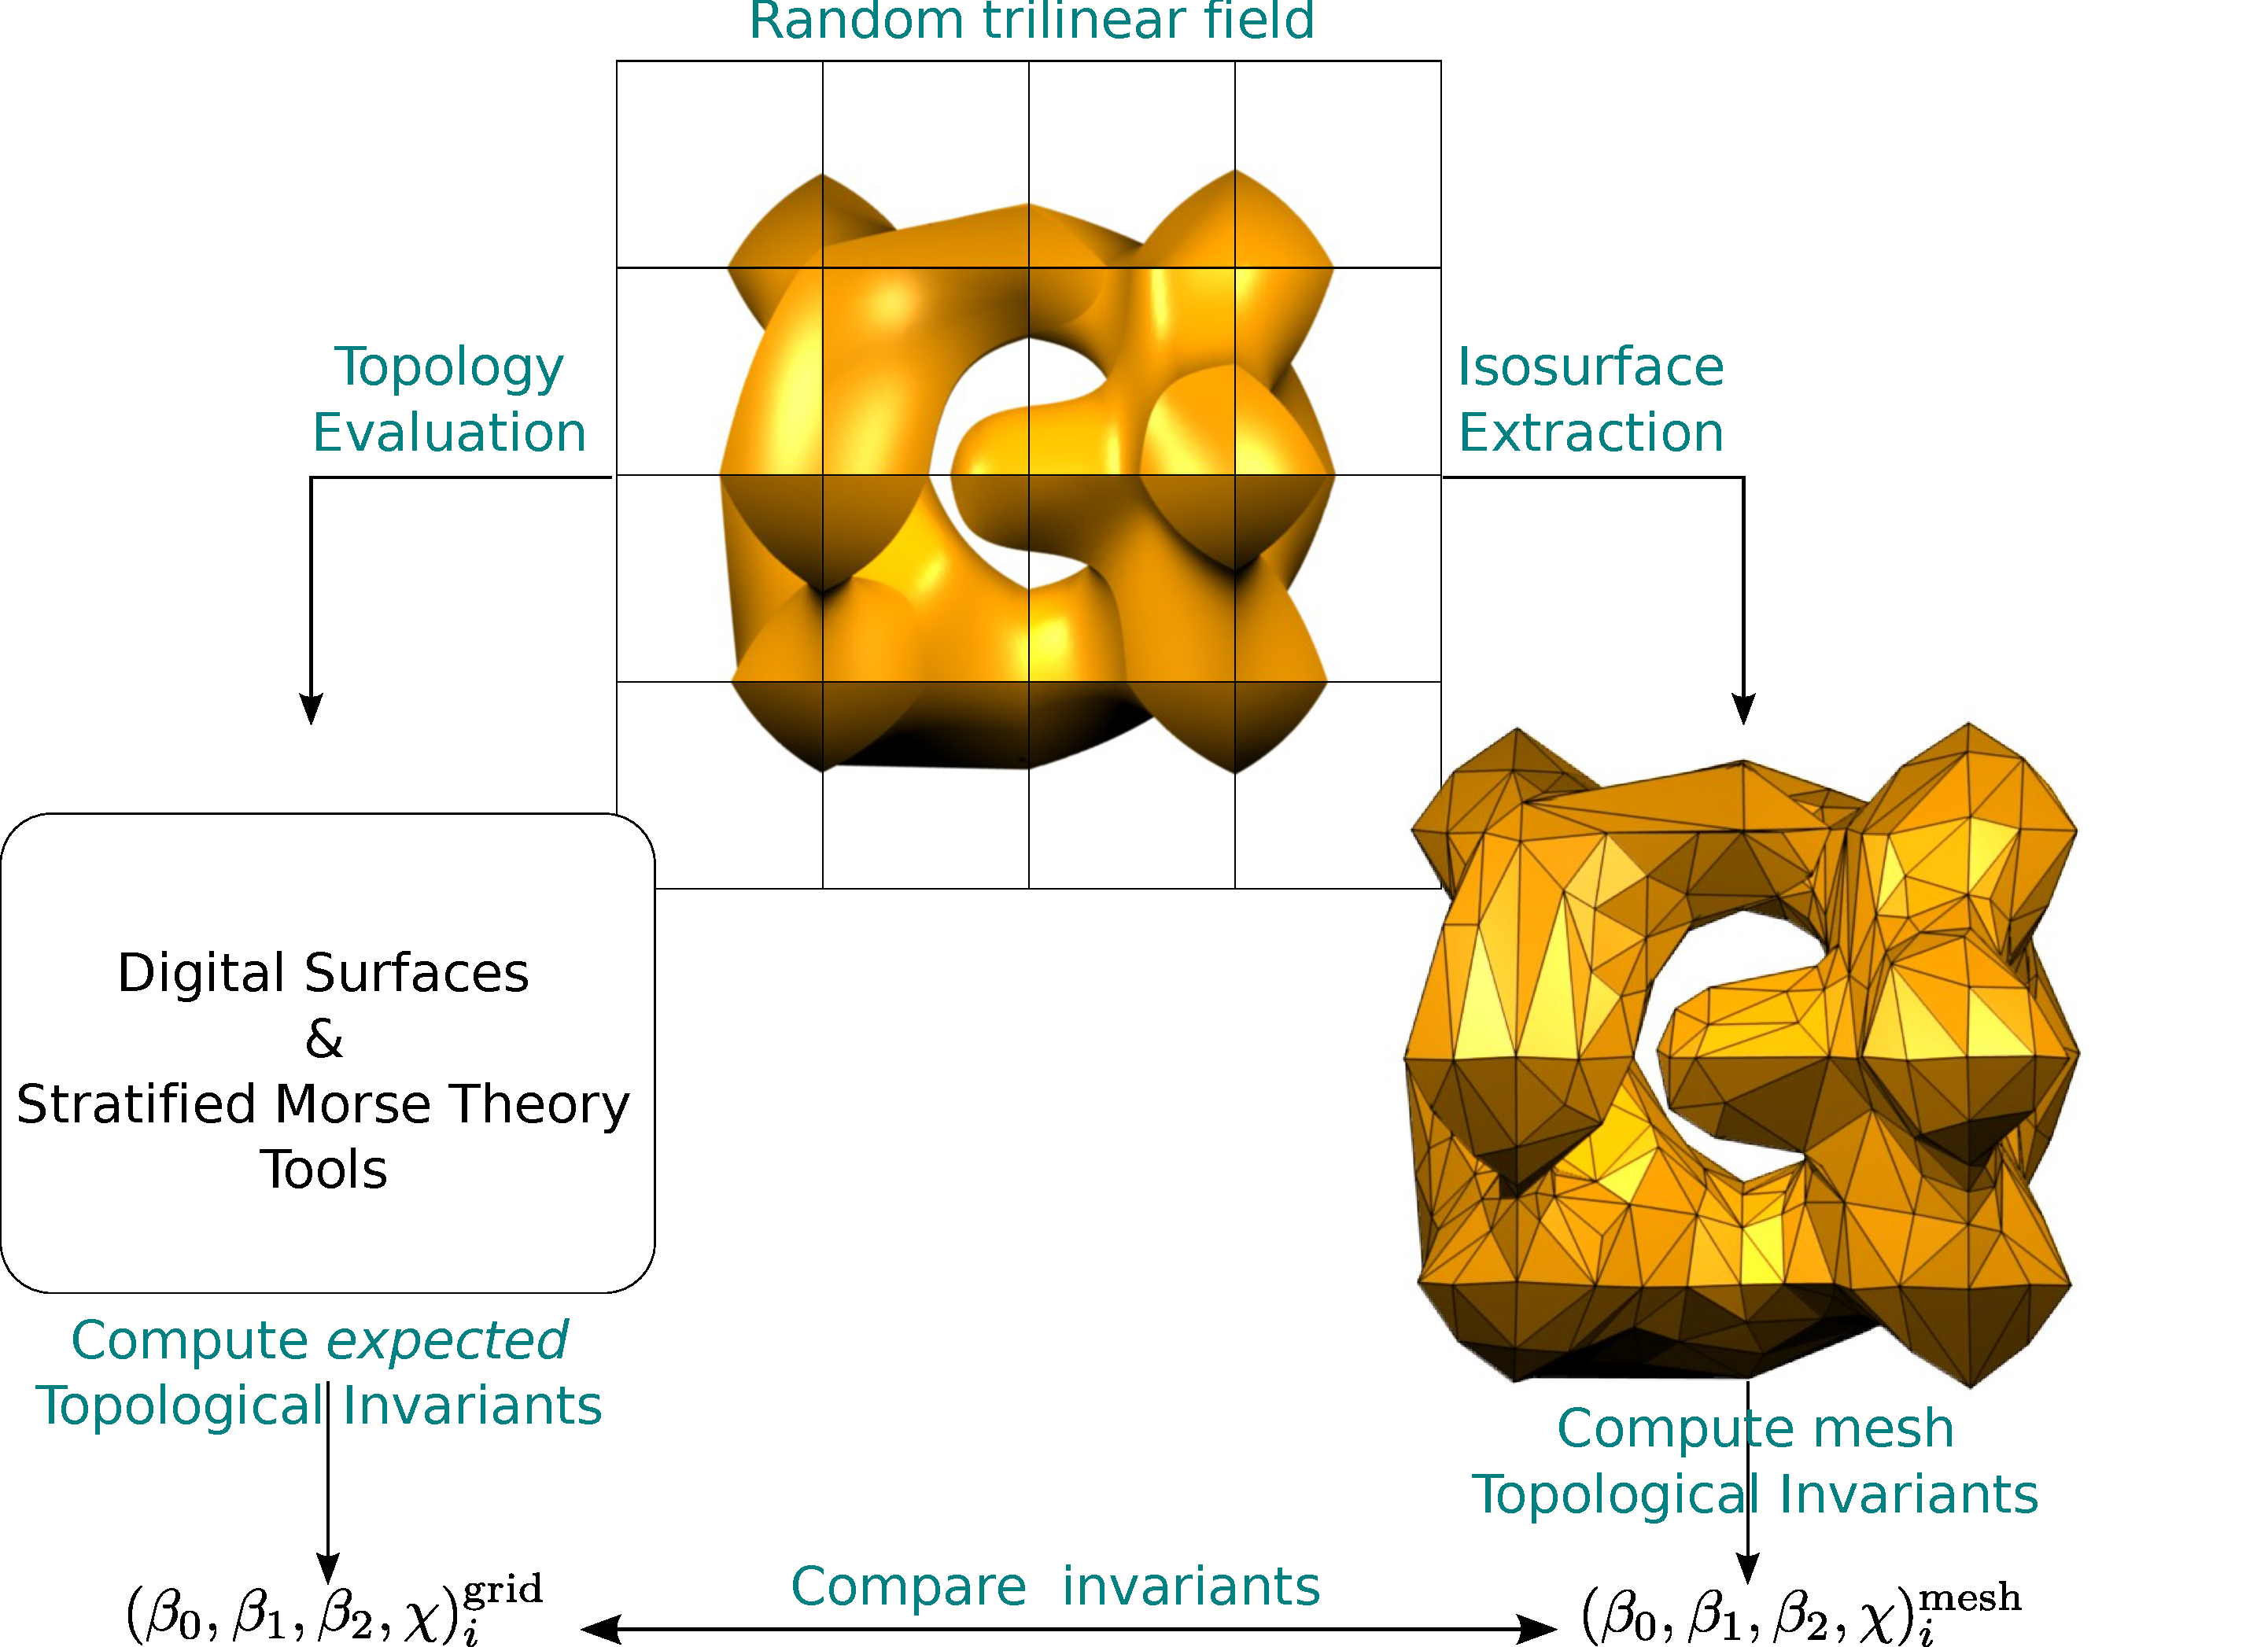
\includegraphics[width=1.0\linewidth,keepaspectratio=true]{chapter3/figures/pipeline.pdf}
\caption{Overview of our topology verification pipeline. First step,
  we generate a random trilinear field and extract a random isosurface
  using the implementation under verification. We then compute the
  \emph{expected} topological invariants from the trilinear field and
  compare them against the invariants obtained from the mesh. We
  provide two simple ways to compute topological invariants from a
  trilinear field based on digital topology (DT) or stratified Morse
  theory (SMT). }
\label{fig:pipeline}
\end{center}
\end{figure}

\section{Mathematical Tools}
\label{sec:math-foundations}

This section describes the mathematical machinery used to derive the
topology verification tools. More specifically, we provide a summary
of the results we need from digital topology and stratified Morse
theory.  A detailed discussion on digital topology can be found in
Stelldinger \emph{et al.}'s paper~\cite{siqueira:2007}, and Goresky and
MacPherson give a comprehensive presentation of stratified Morse
theory~\cite{Goresky:1988:SMT}.

In Section~\ref{sec:digital-topology}, we describe a method, based on
digital topology, that operates on manifold surfaces without
boundaries and determines the Euler characteristic and Betti numbers
of the level sets. A more general setting of surfaces with boundaries
is handled with tools derived from stratified Morse theory, detailed
in Section~\ref{sec:smt}.  The latter method can only determine the
Euler characteristic of the level set.

Let us start by recalling the definition and some properties of the
Euler characteristic, which we denote by $\chi$. For a compact
2-manifold $\mathcal{M}$, $\chi(\mathcal{M}) = V - E + F$, where $V$,
$E$, and $F$ are the number of vertices, edges, and faces of any finite
cell decomposition of $\mathcal{M}$. If $\mathcal{M}$ is a connected
orientable 2-manifold without boundary, $\chi(\mathcal{M}) = 2 -
2g(\mathcal{M})$, where $g(\mathcal{M})$ is the genus of
$\mathcal{M}$. The Euler characteristic may also be written as
$\chi(\mathcal{M}) = \sum_{i=0}^n(-1)^i \beta_i$, where $\beta_i$ are
the Betti numbers: the rank of the $i$-th homology group of
$\mathcal{M}$.
%$\beta_i = \text{rank} H_i(M)$ is the Betti number and $H_i(M)$ is
%the $i^{th}$ Homology group.
Intuitively, for 2-manifolds, $\beta_0$, $\beta_1$ and $\beta_2$
correspond to the number of connected components, holes and voids
(regions of the space enclosed by the surface) respectively.  If
$\mathcal{M}$ has many distinct connected components, that is,
$\mathcal{M} = \bigcup^n_{i = 1} \mathcal{M}^i$ and $\mathcal{M}^i
\bigcap \mathcal{M}^j = \emptyset$ for $i \neq j$ then
$\chi(\mathcal{M}) = \sum_{i}^n \chi(\mathcal{M}^i)$. More details
about Betti numbers, the Euler characteristic, and homology groups can
be found in Edelsbrunner and Harer's text~\cite{edelsbrunner10}. The
Euler characteristic and the Betti numbers are topological invariants:
two homeomorphic topological spaces will have the same Euler
characteristic and Betti numbers whenever these are well-defined.


\subsection{Digital topology}
\label{sec:digital-topology}

Let $\mathcal{G}$ be an $n\times n \times n$ cubic regular grid with a
scalar $e(s)$ assigned to each vertex $s$ of $\mathcal{G}$ and
$t:\mathbb{R}^3\rightarrow\mathbb{R}$ be the piecewise trilinear
interpolation function in $\mathcal{G}$, that is, ~~$t(x) = t_i(x)$,
where $t_i$ is the trilinear interpolant in the cubic cell $c_i$
containing $x$.
%
Given a scalar value $\alpha$, the set of points satisfying
$t(x)=\alpha$ is called the \emph{isosurface} $\alpha$ of $t$. In what
follows, $t(x)=\alpha$ will be considered a compact, orientable
2-manifold without boundary.
%The complement of a cubic cell $c_i$ is a cubic cell $\bar{c}_i$ such
%that for each vertex $s_i \in c_i$ and $\bar{s}_i \in \bar{c}_i$ we
%have $e(\bar{s}_i) < \alpha$ if $ e(s_i) > \alpha$ and $e(\bar{s}_i)
%> \alpha$ if $ e(s_i) < \alpha$.
We say that a cubic cell $c_i$ of $\mathcal{G}$ is \emph{unambiguous}
if the following two conditions hold simultaneously:
\begin{enumerate}
\item any two vertices $s_a$ and $s_b$ in $c_i$ for which
  $e(s_a)<\alpha$ and $ e(s_b)<\alpha$ are connected by \emph{negative
  edges}, i. e., a sequence of edges $s_as_1,s_1s_2,\ldots,s_ks_b$ in
  $c_i$ whose vertices satisfy $e(s_i)<\alpha$ for $i=1,\ldots, k$ and
\item any two vertices $s_c$ and $s_d$ in $c_i$ for which
  $e(s_c)>\alpha$ and $e(s_d)>\alpha$ are connected by \emph{positive
  edges}, i. e., a sequence of edges $s_cs_1,s_1s_2,\ldots,s_ls_d$ in
  $c_i$ whose vertices satisfy $e(s_i)>\alpha$ for $i=1,\ldots,l$.
\end{enumerate}
 In other words, a cell is unambiguous if all positive vertices form a
 single connected component via the positive edges and, conversely, all
 negative vertices form a single connected component by negative
 edges~\cite{gelder:tog:1994}.  If either property fails to hold, $c_i$ is called \emph{ambiguous}. The top
 row in Figure~\ref{fig:topology_preserving} shows all possible
 unambiguous cases.

\begin{figure}[t]
\begin{center}
\includegraphics[width=1\linewidth,keepaspectratio=true]{chapter3/figures/mi.pdf}
\caption{An illustration of the relation between unambiguous
  isosurfaces of trilinear interpolants and the corresponding digital
  surfaces.  The top row shows all possible configurations of the
  intersection of $t = \alpha$ with a cube $c_j$ for unambiguous
  configurations \cite{lopes:tvcg:2003}.  Each red dot $s_i$ denotes a
  vertex with $e(s_i) < \alpha$. Each image on the top right is the
  complement $\bar{c}_i$ of cases 1 to 4 on the left (cases 5 to 7
  were omitted because the complement is identical to the original
  cube up to symmetry).  The middle row shows the volume reconstructed
  by Majority Interpolation (MI) for configurations 1 to 7 (left) and
  the complements (right) depicted in the top row.  Bottom row shows
  the boundary of the volume reconstructed by the MI algorithm (The
  role of faces that intersect $c_i$ is explained in the proof of
  Theorem~\ref{thm:topological_equivalence_trilinear}).  Notice that
  all surfaces in the top and bottom rows are topological disks. For
  each cube configuration, the boundary of each digital reconstruction
  (bottom row) has the same set of positive/negative connected components as the
  unambiguous configurations (top row).  }
\label{fig:topology_preserving}
\end{center}
\end{figure}

The geometric dual of $\mathcal{G}$ is called the \emph{voxel grid}
associated with $\mathcal{G}$, denoted by $V_{\mathcal{G}}$. More
specifically, each vertex $s$ of $\mathcal{G}$ has a corresponding
voxel $v_s$ in $V_{\mathcal{G}}$, each edge of $\mathcal{G}$
corresponds to a face in $V_{\mathcal{G}}$ (and vice versa), and each
cubic cell in $\mathcal{G}$ corresponds to a vertex in
$V_{\mathcal{G}}$, as illustrated in Figure~\ref{fig:voxelgrid}.  Each
voxel $v_s$ can also be seen as the Voronoi cell associated with $s$.
Scalars defined in the vertices of $\mathcal{G}$ can naturally be
extended to voxels, thus ensuring a single scalar value $e(v_s)$ to
each voxel $v_s$ in $V_{\mathcal{G}}$ defined as $e(s)=e(v_s)$.  As we
shall show, the voxel grid structure plays an
important role when using digital topology to compute topological
invariants of a given isosurface. Before showing that relation,
though, we need a few more definitions.

\begin{figure}[t]
\centering
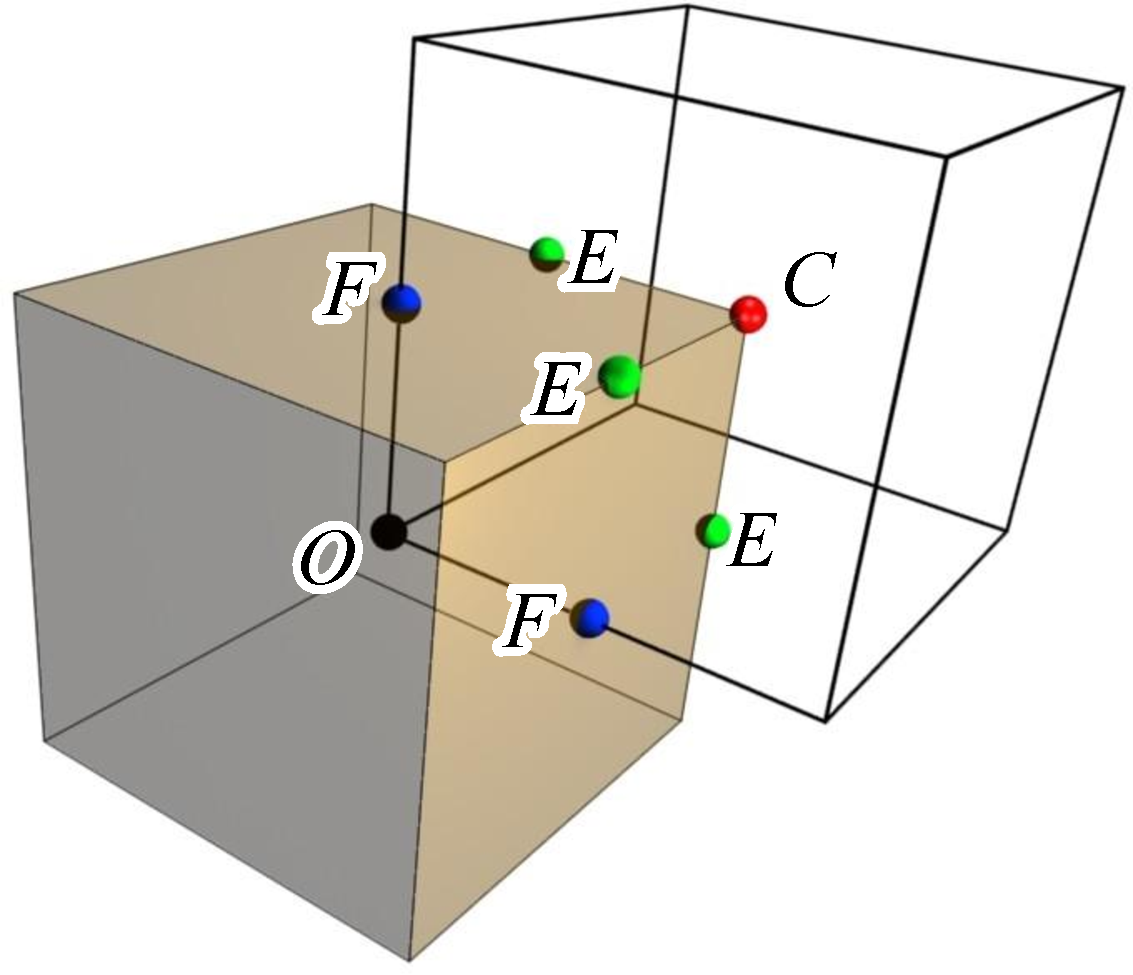
\includegraphics[width=0.35\linewidth]{chapter3/figures/voxel.pdf}
\caption{The four distinct groups of vertices $O, F, E, C$, are
  depicted as black, blue, green, and red points. They are the ``Old'',
  ``Face'', ``Edge,'' and ``Corner'' points of a voxel region
  $V_\mathcal{G}$ (semitransparent cube) respectively. For the sake of
  clarity, we only show a few points.}  
\label{fig:voxelgrid}
\end{figure}


Denote by $\mathcal{G}^\prime$ the $(2n-1)\times (2n-1) \times (2n-1)$ regular grid
obtained from a refinement of $\mathcal{G}$.
%Scalar values can be defined on the vertices of $\mathcal{G}^\prime$
% using the The piecewise trilinear function $t$ defined above, that
% is, if a vertex $s\in\mathcal{G}^\prime$ is also a vertex of
% $\mathcal{G}$ then the value of $e(s)$ is the same as in
% $\mathcal{G}$ otherwise $s$ lies in a cubic cell $c_i$ of
% $\mathcal{G}$ and $e(s)=t(s)$.
Vertices of $\mathcal{G}^\prime$ can be grouped in four distinct sets,
denoted by $O$, $F$, $E$, $C$. The set $O$ contains the vertices of
$\mathcal{G}^\prime$ that are also vertices of $\mathcal{G}$. The sets
$F$ and $E$ contain the vertices of $\mathcal{G}^\prime$ lying on the
center of faces and edges of the voxel grid $V_{\mathcal{G}}$,
respectively. Finally, $C$ contains all vertices of $V_{\mathcal{G}}$.
Figure~\ref{fig:voxelgrid} illustrates these sets.

Consider now the voxel grid $V_{\mathcal{G^\prime}}$ dual to the
refined grid $\mathcal{G}^\prime$.  Given a scalar value $\alpha$, the
\emph{digital object} $\mathcal{O}_\alpha$ is the subset of voxels $v$
in $V_{\mathcal{G^\prime}}$ such that $v\in\mathcal{O}_\alpha$ if at
least one of the criteria below are satisfied:
\begin{itemize}
\item $v\in O$ and $e(v)\leq\alpha$
\item $v\in F$ and both neighbors of $v$ in $O$ have scalars less than
  (or equal to) $\alpha$
\item $v\in E$ and at least $4$ of the $8$ neighbors of $v$ in $O\cup
  F$ have scalars less than (or equal) $\alpha$
\item $v\in C$ and at least $12$ of the $26$ neighbors of $v$ in
  $O\cup F\cup E$ have scalars less than (or equal) $\alpha$
\end{itemize}
The description above is called Majority Interpolation (MI) 
(Algorithm~\ref{alg:majority-interpolation}), and it allows us to compute
the voxels that belong to a digital object $\mathcal{O}_\alpha$.
%satisfying the above criteria, we use Majority Interpolation (MI), a
%procedure illustrated in Figure~\ref{alg:majority-interpolation}.
%cscheid: I removed the sentence below, because it was in the way of
%the rest of the exposition here. It belongs in the discussion More
%importantly, MI is a simple algorithm, an essential requirement in
%the context of verification.
The middle row of Figure~\ref{fig:topology_preserving} shows all
possible cases for voxels picked by the MI algorithm (notice the
correspondence with the top row of the same figure).

\begin{algorithm}[t]
\begin{codebox}
\Procname{$\proc{MajorityInterpolation}(\mathcal{G},\alpha)$}
%\li \Comment Let $S'$ be $S$ with resolution doubled
\li \Comment Let $O$, $F$, $E$ and $C$ be the subset of vertices 
\zi ~~~in $\mathcal{G}^\prime$ as described in
subsection~\ref{sec:digital-topology}. %an old, face, edge and corner point
%\zi  respectively (Definition \ref{dff:majority-interpolation}).
\li \Comment Let $\mathpzc{N}(s, \star)$ be the set of neighbors of
$s\in\mathcal{G}^\prime$ in the \zi ~~~ set $\star$, where $\star =
\{O, F, E, C\}$, with associate scalar \zi ~~~ less than $\alpha$
%\zi of $s \in S'$ inside $p = 0$
\li \For $s \in \mathcal{G}^\prime$
\li     \Do  	\If $s \in O$ \bf or
\li		    $s \in \proc{F}$ and $|\mathpzc{N}(s, O)| = 2$ \bf or
\li			  $s \in E$ and $|\mathpzc{N}(s, O)+\mathpzc{N}(s, F)| 
\geqslant 4$ \bf or
\li		    $s \in \proc{C}$ and $|\mathpzc{N}(s, O)+\mathpzc{N}(s,
F)+\mathpzc{N}(s,E)| \geqslant 12$
\li		\Then Select voxel $v_s$
		\End
	\End
\li \Return $\mathcal{O}_\alpha$
\end{codebox}
\caption{Voxel selection using Majority Interpolation (MI).
}
\label{alg:majority-interpolation}
\end{algorithm}

The importance of $\mathcal{O}_\alpha$ is two-fold. First, the
boundary surface of the union of the voxels in $\mathcal{O}_\alpha$,
denoted by $\partial\mathcal{O}_\alpha$ and called a \emph{digital
  surface}, is a $2$-manifold (See the proof by Stelldinger et
al.~\cite{siqueira:2007}). Second, the genus of
$\partial\mathcal{O}_\alpha$ can be computed directly from
$\mathcal{O}_\alpha$ using the algorithm proposed by Chen and Rong
\cite{LiChen:2008} (Algorithm~\ref{alg:compute-invariant}). As the
connected components of $\mathcal{O}_\alpha$ can also be easily
computed and isolated, one can calculate the Euler characteristic of
each connected component of $\mathcal{O}_\alpha$ from the formula
$\chi = 2 - 2g$ and thus $\beta_0$, $\beta_1$, and $\beta_2$.
% cscheid: We should say how that is done here.

The voxel grid $V_{\mathcal{G^\prime}}$ described above allows us to
compute topological invariants for any digital surface
$\partial\mathcal{O}_\alpha$. However, we so far do not have any
result relating $\partial\mathcal{O}_\alpha$ to the isosurface
$t(x)=\alpha$.  The next theorem provides the connection.

\begin{thm}
Let $\mathcal{G}$ be an $n\times n\times n$ rectilinear grid with scalars
associated with each vertex of $\mathcal{G}$ and $t$ be the piecewise trilinear 
function defined on $\mathcal{G}$, such that the isosurface $t(x)=\alpha$ is a
2-manifold without boundary. If no cubic cell of $\mathcal{G}$ is
ambiguous with respect to $t(x)=\alpha$, then $\partial\mathcal{O}_\alpha$
is homeomorphic to the isosurface $t(x)=\alpha$.
\label{thm:topological_equivalence_trilinear}
\end{thm}
{\bf Proof:} Given a cube $c_i \subset \mathcal{G}$ and an isosurface
 $t = \{x \;|\; t(x) = \alpha\}$, let $t_i = t \cap c_i$.  Similarly,
denote
\[\partial \mathcal{O}_i =  cl_{\mathbb{R}^3} \left( (\partial \mathcal{O}_\alpha \cap c_i) - \partial c_i  \right),\]
where $cl_{\mathbb{R}^3}$ denotes the closure operator. We note that
$\partial \mathcal{O}_i$ is a 2-manifold for all $i$
\cite{SPB04,siqueira:2007}.  There are two main parts to the proof
presented here. For each $i$,
\begin{enumerate}
%\vspace{-0.1in}
\item the 2-manifolds $t_i$ and $\partial \mathcal{O}_i$ are homeomorphic; and
%\vspace{-0.1in}
\item both $t_i$ and $\partial \mathcal{O}_i$ cut the same edges and faces of $c_i$.
%\vspace{-0.1in}
\end{enumerate}

Since $t$ is trilinear, no level-set of $t$ can intersect an edge more
than once. Hence, if $c_i$ is not ambiguous, $t_i$ is exactly one of
the cases 1 to 7 in the top row of
Figure~\ref{fig:topology_preserving}~\cite{lopes:tvcg:2003},
either a topological disk or the empty set.  
%
%The digital reconstruction of each unambiguous case is shown in the
%middle row of Figure \ref{fig:topology_preserving}.
%
Each case in the top row of Figure \ref{fig:topology_preserving} is
the unambiguous input for the MI algorithm to produce the voxel
reconstruction shown in the middle row, where the boundaries of each of
these voxel reconstructions are shown in the bottom row.
%
By inspection, we can verify
that the boundary of the digital reconstruction $\partial
\mathcal{O}_i$ (bottom row of Figure \ref{fig:topology_preserving}) is
also a disk for all possible unambiguous cases and complement cases.
Hence, for each $i$, the 2-manifolds $\partial \mathcal{O}_i$ and
$t_i$ are homeomorphic.
%
Then, for each $i$, both $\partial \mathcal{O}_i$ and $t_i$ cut the same
set of edges and faces of $c_i$. Again, we can verify this for all possible $i$
by inspecting the top and bottom rows in Figure \ref{fig:topology_preserving}, respectively.
%
Finally, we apply the Pasting Lemma~\cite{Munkres} across
neighboring surfaces $\partial \mathcal{O}_i$ and $\partial \mathcal{O}_j$ in order to
establish the homeomorphism between $\partial \mathcal{O}_\alpha$
and $t$.
$\Box$
% cscheid: I don't think the Pasting Lemma applies here. The pasting
% lemma is used to create continuous functions in unions of sets by
% combining continuos functions in the subsets and using the natural
% topology. This is not what we need here - since we are trying to
% relate different subsets (the digital reconstructions and the level
% sets of the scalar field) by homeomorphisms. We need something
% stronger. Our other paper has a lemma that might be too strong, but
% is certainly sufficient.

This proof provides a main ingredient for
the verification method in Section~\ref{sec:manufactured}. Crucially, 
we will show how to manufacture a complex solution that
unambiguously crosses every cubic cell of the grid. Since we have
shown the conditions for which the digital surfaces and the level sets
are homeomorphic, any topological invariant will have to be the
same for both surfaces.

\subsection{Stratified Morse Theory}
\label{sec:smt}
The mathematical developments presented above allow us to compute the
Betti numbers of any isosurface of the piecewise trilinear
interpolant.  However, they require isosurfaces without boundaries.
In this section, we provide a mechanism to compute the Euler
characteristic of any regular isosurface of the piecewise trilinear
interpolant through an analysis based on critical points, which can be
used to verify properties of isosurfaces with boundary components.  We
will use some basic machinery from stratified Morse theory (SMT),
following the presentation of Goresky and MacPherson's
monograph~\cite{Goresky:1988:SMT}.
%We follow the presentation of a separate
%report~\cite{scheidegger:techreport:2010} (submitted as supplementary
%material), which provides a mechanism to compute the Euler
%characteristic of piecewise trilinear isosurfaces using a
%mathematical framework derived from Stratified Morse Theory (SMT)
%\cite{scheidegger:techreport:2010}.

Let $f$ for now be a smooth function with isolated critical points
$p$, where $\nabla f(p) = 0$.  From classical Morse theory, the
topology of two isosurfaces $f(x)=\alpha$ and $f(x)=\alpha+\epsilon$
differs only if the interval $[\alpha, \alpha + \epsilon]$ contains a
critical value ($f(p)$ is a critical value iff $p$ is a critical
point). Moreover, if $\varepsilon_p$ is a small neighborhood around
$p$ and $L^-(p)$ and $L^+(p)$ are the subset of points on the boundary
of $\varepsilon_p$ satisfying $f(x)<f(p)$ and $f(x)>f(p)$
respectively, then the topological change from the isosurface
$f(x)=f(p)-\epsilon$ to $f(x)=f(p)+\epsilon$ is characterized by
removing $L^-(p)$ and attaching $L^+(p)$. Thus, changes in the Euler
characteristic, denoted by $\Delta\chi(p)$, are given by:
\begin{equation}
\Delta\chi(p) = \chi(L^+(p)) - \chi(L^-(p)).
\label{eq:deltachi}
\end{equation}
% \noindent where $\chi(L^-(p))$ and $\chi(L^+(p))$ are the Euler characteristic of $L^-(p)$ and $L^+(p)$,
% respectively. 
\noindent For a smooth function $f$, the number of negative eigenvalues of the
Hessian matrix determines the index of a critical point $p$, and the
four cases give the following values for $\chi(L^-(p))$
and $\chi(L^+(p))$:
%In the smooth scenario, $\chi(L^-(p))$ and $\chi(L^+(p))$
%can be inferred from the number of negative eigenvalues of the Hessian
%matrix of $f$ in $p$, and we have four distinct cases:
\begin{center}
\begin{tabular}{c|c|c|c|c}
& min & saddle-1 & saddle-2 & max \\
\hline
$\chi(L^-(p))$ & 0 & 2 & 0 & 2 \\ 
$\chi(L^+(p))$ & 2 & 0 & 2 & 0
\end{tabular}
\end{center}
The above formulation is straightforward but unfortunately cannot be directly applied to
functions appearing in either piecewise trilinear interpolations or
isosurfaces with boundary, both of which
appear in some of the isosurfacing algorithms with guaranteed
topology. Trilinear interpolants are not smooth across the faces
of grid cells, so the gradient is not well-defined there. Identifying the
critical points using smooth Morse theory is then
problematic. Although arguments based on smooth Morse
theory have appeared in the
literature~\cite{Weber:2002:ESF}, there are complications. For
example, the scalar field in a node
of the regular grid might not have \emph{any} partial
derivatives. Although one can still argue about the
intuitive concepts of minima and maxima around a non-differentiable point,
configurations such as saddles are more problematic, since their
topological behavior is different depending on whether they are on the
boundary of the domain. It is 
important, then, to have a mathematical tool which makes predictions
regardless of the types of configurations, and SMT is one such theory.

Intuitively, a \emph{stratification} is a partition of a
piecewise-smooth manifold such that each subset, called a
\emph{stratum}, is either a set of discrete points or has a smooth
structure.  In a regular grid with cubic cells, the stratification we
propose will be formed by four sets (the strata), each one a (possibly
disconnected) manifold.  The \emph{vertex set} contains all vertices
of the grid. The \emph{edge set} contains all edge interiors, the
\emph{face set} contains all face interiors, and the \emph{cell set}
contains all cube interiors. We illustrate the concept for the 2D case
in Figure~\ref{fig:stratification}.  The important property of the
strata is that the level sets of $f$ restricted to each stratum are
smooth (or lack any differential structure, as in the vertex-set). In
SMT, one applies standard Morse theory on each stratum, and then
combines the partial results appropriately.

\begin{figure}[t]
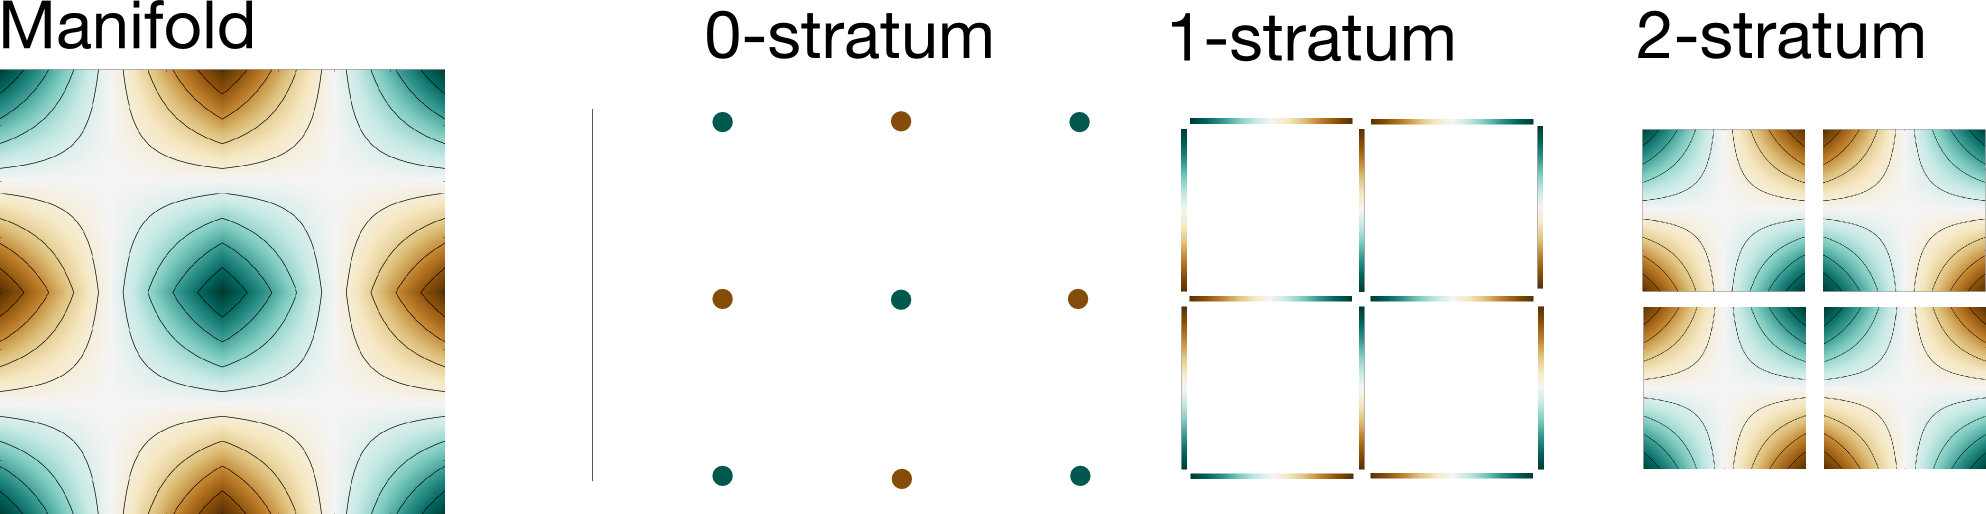
\includegraphics[width=\linewidth]{chapter3/figures/stratification.png}
\caption{\label{fig:stratification}An illustration of a
  piecewise-smooth immersed 2-manifold. The colormap illustrates the
  value of each point of the scalar field. Notice that although the manifold
  itself is not everywhere differentiable, each stratum is itself an open
  manifold that is differentiable.}
\end{figure}

The set of points with zero gradient (computed on each stratum), which
SMT assumes to be isolated, are called the \emph{critical points} of
the stratified Morse function. In addition, every point in the vertex
set is considered critical as well. One major difference between SMT
and the smooth theory is that some critical points do not actually
change the topology of the level sets. This is why considering all
grid vertices as critical does not introduce any practical problems:
most grid vertices of typical scalar fields will be \emph{virtual
  critical points}, {\em i.e.}, points which do not change the Euler
characteristic of the surface. Carr and Snoeyink use a
related concept (which they call ``potential critical points'') in
their state-machine description of the topology of
interpolants~\cite{CS08}.

Let $\mathcal{M}$ be the stratified grid described above.  It can be
shown that if $p$ is a point in a $d$-dimensional stratum of
$\mathcal{M}$, it is always possible to find a $(3-d)$-dimensional
submanifold of $\mathcal{M}$ (which might straddle many strata) that
meets transversely the stratum containing $p$, and whose intersection
consists of only $p$ (one way to think of this $(3-d)$-manifold is as a ``topological orthogonal
complement'').  In this context, we can define a small neighborhood
$T_\varepsilon(p)$ in the strata containing $p$ and the \emph{lower
  tangential} link $T_L^-(p)$ as the set of points in the boundary of
$T_\varepsilon(p)$ with scalar values less than that in $p$ (see Figure \ref{fig:chap4:smt}).
\begin{figure}[b]
\centering
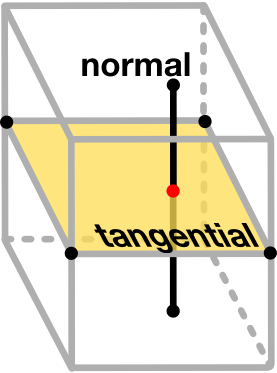
\includegraphics[width=0.3\linewidth]{chapter3/figures/ilustration.png}
\caption{\label{fig:chap4:smt} Example of tangential and normal link.}
\end{figure}
Similarly we can define the \emph{upper tangential} link $T_L^+(p)$ as
the set of points in the boundary of $T_\varepsilon(p)$ with scalar
value higher than that at $p$.  \emph{Lower normal} $N_L^-(p)$ and
\emph{upper normal} $N_L^+(p)$ links are analogous notions, but the
lower and upper links are taken to be subsets of $N_\varepsilon(p)$,
itself a subset of the $(3-d)$-dimensional submanifold transverse to
the stratum of $p$ going through $p$.  The definitions above are needed
in order to define the \emph{lower stratified link} and \emph{upper
  stratified link}, as follows: given $T_\varepsilon(p),\,
T_L^-(p),\,N_\varepsilon(p)$ and $N_L^-(p)$, the \emph{lower
  stratified Morse link} (and similarly for upper stratified link) is
given by
\begin{equation}
L^-(p) = (T_\varepsilon(p) \times N_L^-(p)) \cup (N_\varepsilon(p)
\times T_L^-(p)) \label{eq:lowerstratifiedlink}.
\end{equation}
These definitions allow us to classify critical points even in the non-smooth scenario.
They let us compute topological changes with
the same methodology used in the smooth case. In other words, when a
scalar value $\alpha$ crosses a critical value $\alpha_p$ in a
critical point $p$, the topological change in the isosurface is
characterized by removing $L^-(p)$ and attaching $L^+(p)$, affecting
the Euler characteristic as defined in Equation~\ref{eq:deltachi}.%\cite{?}.

The remaining problem is how to determine $\chi(L^-(p))$ and
$\chi(L^+(p))$. 
Recalling that $\chi(A \cup B) = \chi(A) + \chi(B) - \chi(A \cap B)$,
$\chi(A\times B)=\chi(A)\chi(B)$, and $\chi(T_\varepsilon)=\chi(N_\varepsilon)=1$ (we are omitting 
the point $p$) we have:
\begin{equation}
\begin{array}{l}
\chi(L^-) = \chi(T_\varepsilon \times N_L^- \cup N_\varepsilon \times T_L^-) \\
    \qquad  = \chi(N_L^-) + \chi(T_L^-) - \chi(T_\varepsilon \times N_L^- \cap N_\varepsilon \times T_L^-)
\end{array}
\end{equation}
Now, we can define $T_\varepsilon = T_L^- \cup T_r,\, T_L^- \cap T_r =
\emptyset$ and similarly for $N_\varepsilon$ and $N_L^-$.  Then,
expand the partitions and products, and distribute the intersections
around the unions, noticing all but one of intersections will be
empty:
\begin{eqnarray*}
T_\varepsilon \times N_L^- \cap N_\varepsilon \times T_L^- \hspace{-8.0px} &=& \hspace{-8.0px} ((T_r \cup T_L^-) \times N_L^-) \cap ((N_r \cup N_L^-) \times T_L^-) \\
\hspace{-8.0px} &=& \hspace{-8.0px} ((T_r \times N_L^-) \cup (T_L^- \times N_L^-)) \cap \\
\hspace{-8.0px} && \hspace{-8.0px}((N_r \times T_L^-) \cup (N_L^- \times T_L^-)) \\
\hspace{-8.0px} &=& \hspace{-8.0px}N_L^- \times T_L^-
\end{eqnarray*}
Therefore:
\begin{eqnarray*}
\chi(T_\varepsilon \times N_L^- \cap N_\varepsilon \times T_L^-) &=& \chi(N_L^- \times T_L^-) \\
&=& \chi(N_L^-)\chi(T_L^-)
\end{eqnarray*}
which gives the final result
\begin{equation}
\chi(L^-) = \chi(N_L^-)+\chi(T_L^-)-\chi(N_L^-)\chi(T_L^-) \label{eq:lowerchi}.
\end{equation}

The same result is valid for $\chi(L^+)$, if we replace the 
superscript `$-$' by `$+$' in Equation~\ref{eq:lowerchi}. If $T_L^-$ or
$T_L^+$ are one-dimensional, then we are done. If not, then we can
recursively apply the same equation to $T_L^-$ and $T_L^+$ and look at
progressively lower-dimensional strata until we reach
$T_\varepsilon(p)$ and $N_\varepsilon(p)$ given by $1$-disks. The
lower and upper links for these \mbox{$1$-disks} will always be
discrete spaces with zero, one, or two points, for which $\chi$ is
simply the cardinality of the set.

In some cases, the Euler characteristic of the lower and upper link
might be equal. Then, $\chi(L^-(p)) = \chi(L^+(p))$, and
$\Delta\chi(p) = 0$. These cases correspond to the virtual critical
points mentioned above.
%, that is, critical points which do not change
%the Euler characteristic of the surface.
%
Critical points in the interior of cubic cells are handled by the
smooth theory, since in that case the normal Morse data is
0-dimensional. This implies that the link will be an empty set with
Euler characteristic zero. So, by Equation~\ref{eq:lowerchi},
$\chi(L^-) = \chi(T_L^-)$. Because the restriction of the scalar field
to a grid edge is a linear function, no critical point can appear
there. As a result, the new cases are critical points occurring at
vertices or in the interior of faces of the grid.  For a critical
point $p$ in a vertex, stratification can be carried out recursively,
using the edges of the cubes meeting in $p$ as tangential and normal
submanifolds. Denoting by $n_{l1},n_{l2},n_{l3}$ the number of
vertices adjacent to $p$ with scalar value less than that of $p$ in
each Cartesian coordinate direction, Equation~(\ref{eq:lowerchi})
gives:
\begin{equation}
\chi(L^-(p)) = n_{l1}+n_{l2}+n_{l3} - n_{l1}(n_{l2}+n_{l3})
\end{equation}
$\chi(L^+(p))$ can be computed similarly, but considering the number of neighbors of $p$ in each Cartesian 
direction with scalars higher than that of $p$.

If $p$ is a critical point lying in a face $r$ of a cube, we consider
the face itself as the tangential submanifold and the line segment
$r^\perp$ orthogonal to $r$ through $p$ the normal submanifold.
Recursively, the tangential submanifold can be further stratified in
two $1$-disks (tangential and normal).  Denote by $n_l$ the number of
ends of $r^\perp$ with scalar value less than that of $p$. Also,
recalling that the critical point lying in the face $r$ is necessarily
a saddle, thus having two face corners with scalar values less and two
higher than that of $p$, Equation~(\ref{eq:lowerchi}) gives:
\begin{equation}
\chi(L^-(p)) = n_l+2 - 2\,n_l
\end{equation}
Analogously, we can compute $\chi(L^+(p)) = n_u+2 - 2\,n_u$ where
$n_u$ is the number of ends of $r^\perp$ with scalar value higher than
that of $p$.

A similar analysis can be be carried out for every type of critical
point, regardless of whether the point belongs to the interior of a
grid cell (and so would yield equally well to a smooth Morse theory
analysis), an interior face, a boundary face, or a vertex of any
type. The Euler characteristic $\chi_\alpha$ of any isosurface with
isovalue $\alpha$ is simply given as:
\begin{equation}
\chi_\alpha = \sum_{p_i\in C_\alpha} \Delta\chi(p_i)
\label{ref:chis}
\end{equation}
where $C_\alpha$ is the set of critical points with critical values less than $\alpha$.

It is worth mentioning once again that, to the best of our knowledge,
no other work has presented a scheme which provides such a simple
mechanism for computing the Euler characteristic of level sets of
piecewise-smooth trilinear functions. Compare, for example, the case
analyses and state machines performed separately by
Nielson~\cite{Nielson03onmarching}, by Carr and Snoeyink~\cite{CS08},
and by Carr and Max~\cite{10.1109/TVCG.2009.10}. In contrast, we can recover an
(admittedly weaker) topological invariant by a much simpler
argument. In addition, this argument already generalizes (trivially
because of the stratification argument) to arbitrary dimensions,
unlike the other arguments in the literature.


\section{Manufactured Solution Pipeline}
\label{sec:manufactured}

We now put the pieces together and build a pipeline for topology 
verification using the results presented in Section~\ref{sec:math-foundations}. 
In the following sections, the procedure called $\proc{Isosurfacing}$ refers to the
isosurface extraction technique under verification.
$\proc{InvariantFromMesh}$ computes topological invariants of a simplicial
complex. 
%Section \ref{sec:discussion} compares the verification pipelines using
%Digital Topology and Stratified Morse Theory.


\subsection{Consistency}
\label{sec:consistency-verification}

As previously mentioned, MC-like algorithms which use
disambiguation techniques are expected to generate PL manifold isosurfaces no matter how complex 
the function sampled in the vertices of the regular grid. 
In order to stress the consistency test, we generate a random scalar field with values in the
interval $[-1,1]$ and extract the isosurface with isovalue $\alpha=0$
(which is all but guaranteed not to be a critical value) using a
given isosurfacing technique, subjecting the 
resulting triangle mesh to the consistency verification. This process
is repeated a large number of times, and  
%
if the implementation fails to
produce \mbox{PL manifolds} for all cases, then the counterexample
provides a documented starting point for debugging. If it passes the
tests, we consider the implementation verified.
% (in the sense of analyzed predicted behavior) for all test cases to which
% it has been applied, increasing our confidence in the stated properties

\subsection{Verification using Stratified Morse Theory}
\label{subsec:smt-verify}

We can use the formulation described in Section~\ref{sec:smt} to
verify isosurfacing programs which promise to match the
topology of the trilinear interpolant.
The SMT-based verification procedure is summarized in
Algorithm~\ref{alg:manufactured-solutions-smt}. The algorithm 
has four main steps. A random scalar field with node values in the
interval $[-1,1]$ is initially created. Representing the trilinear
interpolation in a grid cell by $f(x,y,z) = axyz + bxy + cxz + dyz + ex + fy + gz + h$,
the internal critical points are given by:
\[\begin{array}{ccc}
t_x = (d \Delta_x \pm \sqrt{\Delta_x \Delta_y \Delta_z})/({a \Delta_x})\\
t_y = (c \Delta_y \pm \sqrt{\Delta_x \Delta_y \Delta_z})/({a \Delta_y})\\
t_z = (b \Delta_z \pm \sqrt{\Delta_x \Delta_y \Delta_z})/({a \Delta_z}),
\end{array}\]
%% \begin{eqnarray*}
%% t_x &=&  \\
%% t_y &=&  \\
%% t_z &=&  
%% \end{eqnarray*}
\noindent where $\Delta_x = bc-ae$, $\Delta_y = bd-af$, and $\Delta_z
= cd-ag$~\cite{Pascucci03}.  Critical points on faces of the cubes are found by setting
$x,y$ or $z$ to either 0 or 1, and solving
the quadratic equation.  
If the solutions lie outside the unit cube $[0, 1]^3$, they are not
considered critical points, since they lie outside the domain of the cell. The scalar field
is regenerated if any degenerate critical point is detected (these
can happen if either the random values in a cubic cell have, by chance, the same value or when 
$\Delta_x$, $\Delta_y$ or $\Delta_z$ are zero). In order
to avoid numerical instabilities, we also regenerate the scalar field
locally if any internal critical point lies too close to the border of
the domain (that is, to an edge or to a face of the cube).

\begin{algorithm}[t]
\begin{codebox}
\Procname{$\proc{MMS-SMT}(\mathcal{G})$}
\li \Comment Let the input $\mathcal{G}$ be $n \times n \times n$ rectilinear grid
\li \For $i \gets 1$ \To $\#$tests
\li     \Do $\mathcal{G} \gets$ randomly sampled $n \times n \times n$ grid \label{alg:mms:sampling}
\li         $\id{CPs} \gets \proc{ComputeCriticalPoints}(\mathcal{G})$
\li         \If $p \in CPs$ is degenerate \kw{or}
\li		$p$ is an internal saddle close to edges or faces
\li         	\Then $\proc{GoTo}$ \ref{alg:mms:sampling} \label{alg:mms:goto-smt}
\li         \Else $K \gets \proc{Isosurfacing}(\mathcal{G})$
\li         	  $(\chi^v)_i \gets \proc{InvariantFromCPs}(\mathcal{G})$
\li         	  $(\chi^k)_i \gets \proc{InvariantFromMesh}(K)$
	    \End
\li Compare $(\chi^v)_i$ and $(\chi^k)_i$
      \End
\end{codebox}
\caption{Overview of the method of manufactured solutions (MMS) using
stratified Morse theory. \proc{InvariantFromCPs} is computed using Equation
\ref{ref:chis}. The method either fails to match the expected topology, in
which case $\mathcal{G}$ is provided as a counterexample, or
succeeds otherwise.}
\label{alg:manufactured-solutions-smt}
\end{algorithm}

The third step computes the Euler characteristic of a set of
isosurfaces with random isovalues in the interval $[-1, 1]$ using the
theory previously described, jointly with Equation~\ref{ref:chis}.  In
the final step, the triangle mesh $M$ approximating the isosurfaces is
extracted using the algorithm under verification, and $\chi(M) = V(M)
- E(M) + F(M)$, where $V(M),E(M)$, and $F(M)$ are the number of
vertices, edges, and triangles. If the Euler characteristic computed
from the mesh does not match the one calculated via
Equation~\ref{ref:chis}, the verification fails. We carry out the
process a number of times, and implementations that pass the tests are
less likely to contain bugs.

\subsection{Verification using Digital Topology}
\label{subsec:ds-verify}

Algorithm~\ref{alg:manufactured-solutions-digital-surfaces} shows the
verification pipeline using the MI algorithm, and
Figure~\ref{fig:trilinear-field} depicts the refinement process. Once
again a random scalar field, with potentially many ambiguous cubes, is
initially generated in the vertices of a grid $\mathcal{G}$.  The
algorithm illustrated in
Algorithm~\ref{alg:manufactured-solutions-digital-surfaces} is applied to
refine $\mathcal{G}$ so as to generate a new grid
$\tilde{\mathcal{G}}$ which does not have ambiguous cells. If the
maximum number of refinement is reached and ambiguous cells still
remain, then the process is restarted from scratch.  Notice that cube
subdivision does not need to be uniform.  For instance, each cube may
be refined using a randomly placed new node point or using $t_i$'s
critical points, and the result of the verification process still
holds.  This is because Theorem
$\ref{thm:topological_equivalence_trilinear}$ only requires $c_i$ to
be unambiguous.
%This shows us that the reliability of this verification process depends 
%only on key concepts with other steps performed in
%possibly many different ways. 
For simplicity, in this work we refine $\mathcal{G}$ uniformly
doubling the grid resolution in each dimension.

\begin{algorithm}[t]
\begin{codebox}
\Procname{$\proc{MMS-DS}(\mathcal{G})$}
\li \Comment Let the input $\mathcal{G}$ be a $n \times n \times n$ rectilinear grid
\li \For $i \gets 1$ \To $\#$tests
\li     \Do  $\mathcal{G} \gets$ randomly sampled $n \times n \times n$ grid \label{alg:mms:sampling2}
\li         $\tilde{\mathcal{G}} \gets \proc{RefineAndResample}(\mathcal{G})$
\li         \If $\tilde{\mathcal{G}}$ has ambiguous cubes
\li         	\Then $\proc{GoTo}$ \ref{alg:mms:sampling2} \label{alg:mms:goto-dt}
			\End
\li         $\mathcal{O} \gets
\proc{MajorityInterpolation}(\tilde{\mathcal{G}})$
\li 		  $K \gets \proc{Isosurfacing}(\mathcal{G})$
\li         	  $(\beta_0^v, \beta_1^v,\beta_2^v)_i \gets
\proc{InvariantFromDS}(\partial {\mathcal{O}})$
\li         	  $(\beta_0^k, \beta_1^k,\beta_2^k)_i \gets
\proc{InvariantFromMesh}(K)$
\li Compare $(\beta_0^v, \beta_1^v,\beta_2^v)_i$ and $(\beta_0^k, \beta_1^k,\beta_2^k)_i$
	    \End
      \End
\end{codebox}
\caption{Overview of the method of manufactured solutions (MMS) using digital
topology. The method either fails to match the expected topology, in
which case $\mathcal{G}$  is provided as a counterexample, or
succeeds otherwise.}
\label{alg:manufactured-solutions-digital-surfaces}
\end{algorithm}

\begin{figure}[t]
\centering
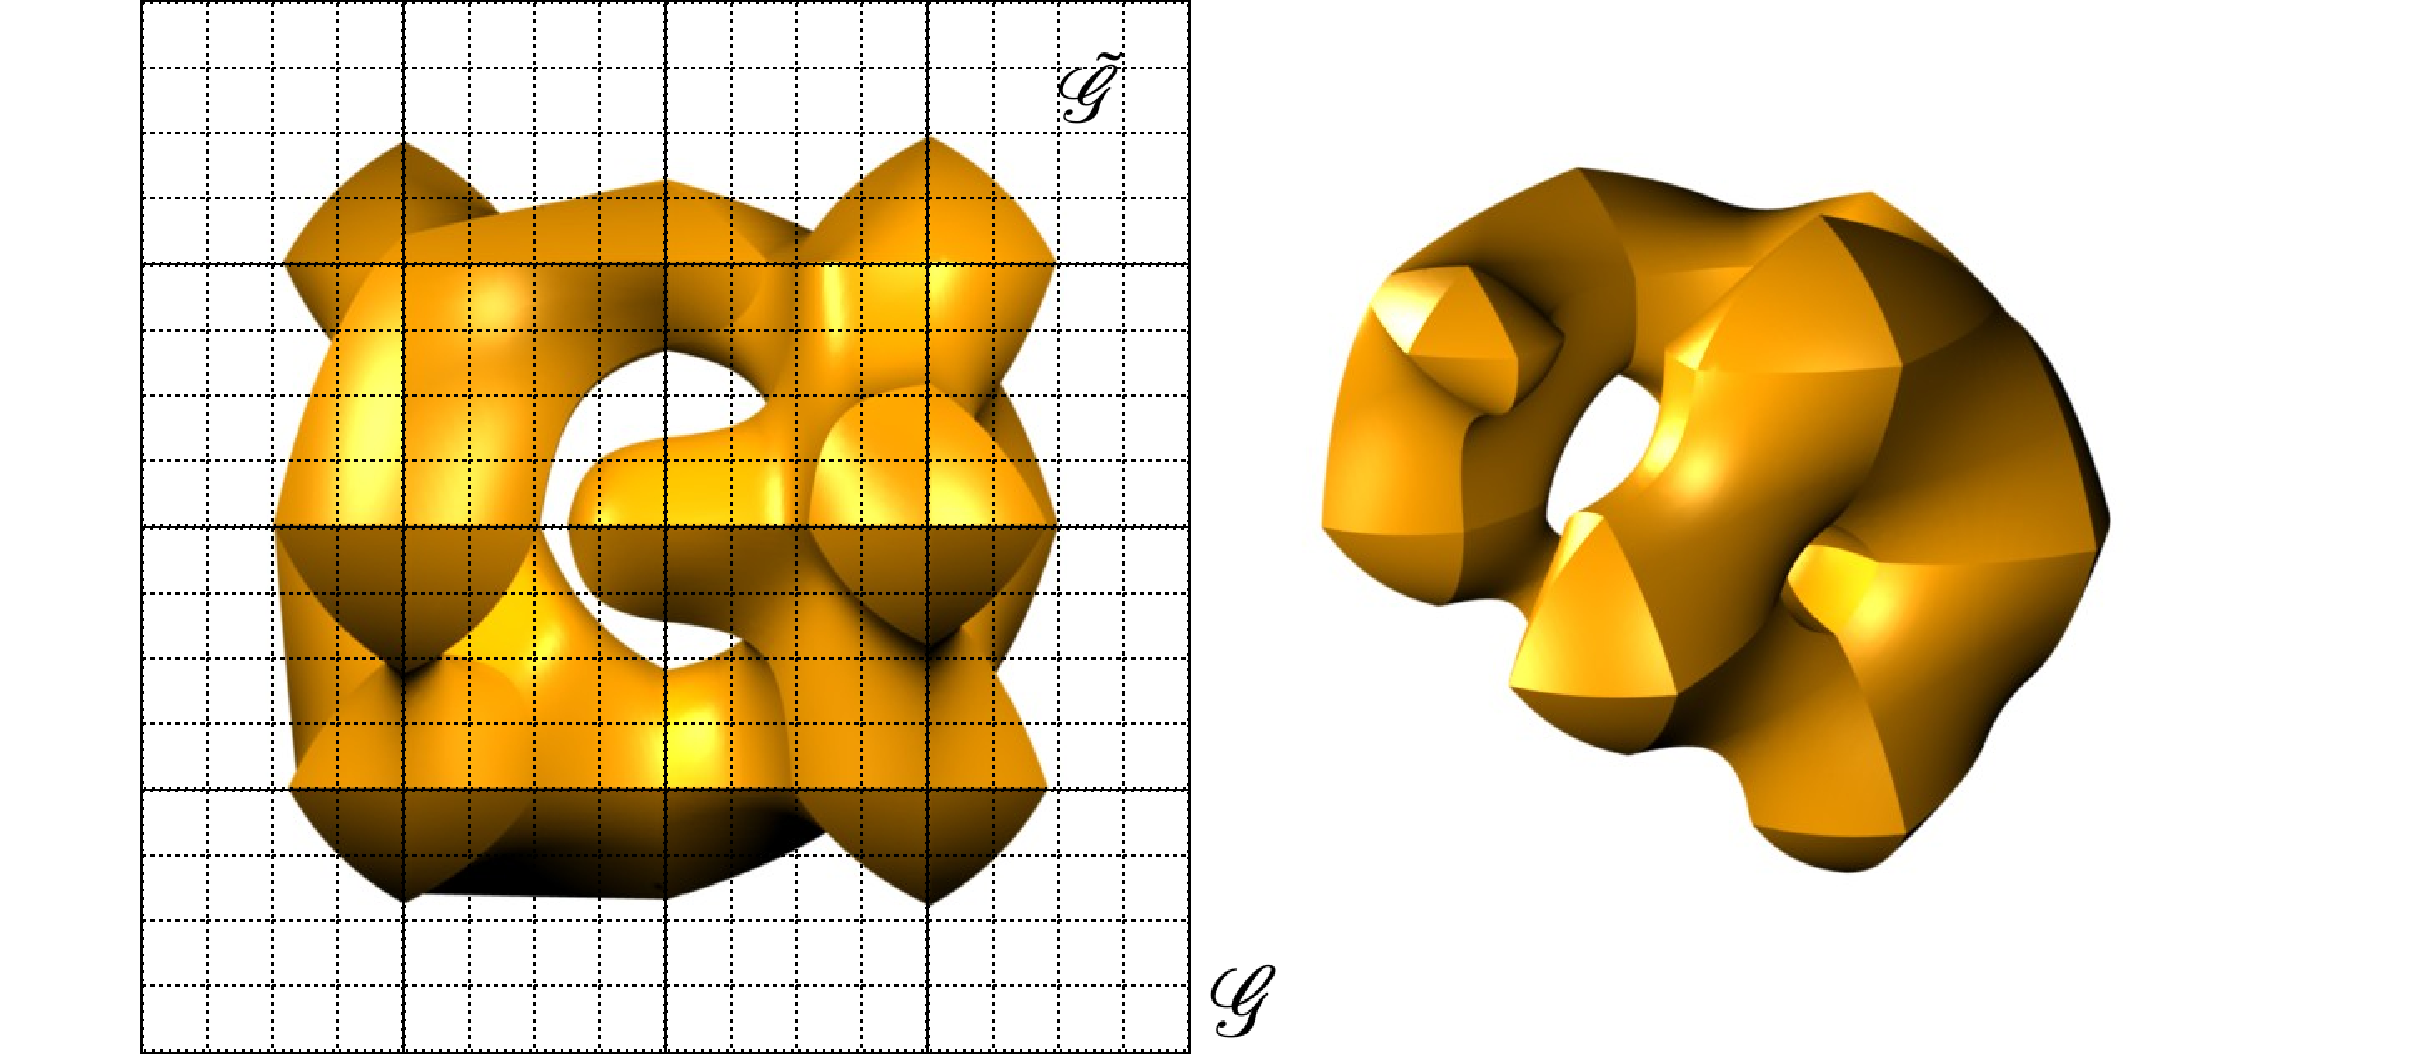
\includegraphics[width=1.0\linewidth,keepaspectratio=true]
{chapter3/figures/trilinear-field.pdf}
\caption{Our manufactured solution is given by $t(x) = \alpha$. $\mathcal{G}$ is
depicted in solid lines while $\tilde{\mathcal{G}}$ is shown in dashed lines.
$\tilde{\mathcal{G}}$ is a uniform subdivision of $\mathcal{G}$. The trilinear
surfaces $t_i$ are defined for each cube
$c_i \in \mathcal{G}$ and resampled in $c'_j \in \tilde{\mathcal{G}}$.
The cubes in the center of $\mathcal{G}$ have four maxima each
(left) and thus induce complicated topology. The final
isosurface may have several tunnels and/or connected
components even for coarse $\mathcal{G}$ (right). }
\label{fig:trilinear-field}
\end{figure}

Scalars are assigned to the new vertices of $\tilde{\mathcal{G}}$ (the ones not in $\mathcal{G}$) by trilinearly 
interpolating
from scalars in $\mathcal{G}$, thus ensuring that $\mathcal{G}$ and  $\tilde{\mathcal{G}}$ have
exactly the same scalar field~\cite{Nielson03onmarching}.
As all cubic cells in $\tilde{\mathcal{G}}$ are unambiguous, Theorem \ref{thm:topological_equivalence_trilinear} guarantees 
the topology of the digital surface $\partial\mathcal{O}_\alpha$
obtained from $\tilde{\mathcal{G}}$ is equivalent to 
that of $t(x)=\alpha$. Algorithm \proc{InvariantFromDS} computes
topological invariants of
$\partial\mathcal{O}_\alpha$ using the scheme discussed in
Section~\ref{sec:digital-topology}. In this context, \proc{InvariantFromDS} is
the algorithm illustrated in Algorithm~\ref{alg:compute-invariant}.
Surfaces with boundary are avoided by assigning the scalar value $1$ to every vertex in the
boundary of $\mathcal{G}$.

\begin{algorithm}[b]
\begin{codebox}
\Procname{$\proc{GenusFromDS}(\partial \mathcal{O}_\alpha)$}
\li \Comment Let $\partial \mathcal{O}_\alpha$ be a 2-manifold without
boundary
\li \Comment Let $|\mathpzc{N}_i|$ be the number of surface points with
\zi ~~~exactly $i$ neighbors.
\li \Comment Let $g$ be the surface genus
\li $g = 1 + (|\mathpzc{N}_5| + 2 |\mathpzc{N}_6| - |\mathpzc{N}_3|) / 8 $
\li \Return $g$
\end{codebox}
\caption{A simple formula for genus computation.}
\label{alg:compute-invariant}
\end{algorithm}


\section{Experimental Results}
\label{sec:results}

In this section, we present the results of applying our topology verification
methodology to a number of different isosurfacing techniques, 
three of them with topological guarantees with respect to trilinear interpolant.
Specifically, the techniques are:

\vtk\ \cite{vtk} is the Visualization Toolkit (VTK) implementation of the
Marching Cubes algorithm with the
implicit disambiguation scheme proposed by Montani \emph{et al.}
\cite{Montani:1994:MLT}. Essentially, it separates positive vertices when a
face saddle appears and assumes no tunnels exist inside a cube. The
proposed scheme is topologically consistent, but it does not reproduce the
topology of the trilinear interpolant. 

Marching Cubes with Edge Transformations or \macet\ \cite{Dietrich:TVCG:2008} is
a Marching Cubes-based technique designed to generate triangle 
meshes with good quality. 
%The authors show that approximately parallel intersections
%between an isosurface and a grid cube are responsible for bad triangle quality.
Quality is reached by displacing active edges of the grid (edges intersected by the
isosurface), both in normal and tangential direction toward avoiding ``sliver'' intersections. 
%The results presented shows substancial improvement on mesh quality. 
Macet does not reproduce the topology of the trilinear interpolant.

\afront~\cite{Schreiner06} is an advancing-front method for isosurface
extraction, remeshing, and triangulation of point sets. It works by advancing
triangles over an implicit surface. A sizing function that takes curvature into account
is used to adapt the triangle mesh to features of the
surface. \afront\ uses cubic spline reconstruction kernels to
construct the scalar field from a regular grid.
%is derived from a Afront's main feature is a
%special scheme for adapting triangle size according to surface curvature.
The algorithm produces high-quality triangle meshes with bounded
Hausdorff error. As occurred with the VTK and Macet implementations, Afront produces consistent
surfaces but, as expected, the results do not match the trilinear
interpolant.

\matlab$^\circledR$ \cite{matlab10} is a high-level language for building codes that requires intensive
numerical computation. It has a number of features and among them an isosurface extraction routine for volume data
visualization. Unfortunately, \matlab\ documentation does not offer information
on the particularities of the implemented isosurface extraction technique (e.g., Marching Cubes, Delaunay-based, etc; consistent or correct).

\snapmc\ \cite{Raman:2008:QIM} is a Marching Cubes variant which produces high-quality 
triangle meshes from regular grids. The central idea is to extend the 
original lookup table to account for cases where the isosurface passes exactly through the 
grid nodes. Specifically, a user-controlled parameter dictates maximum distance 
for ``snapping'' the isosurface into the grid node. 
The authors report an improvement in the minimum triangle angle when compared to previous techniques.


\mclewiner\ was introduced by Chernyaev
\cite{Chernyaev95marchingcubes} to solve ambiguities in the original MC. It
extends Marching Cubes table from 15 to 33 cases to account for ambiguous cases
and to reproduce the topology of the trilinear interpolant inside each cube. The
original table was later modified to remove two redundant cases which leads to 31
unique configurations. Chernyaev's MC solves face ambiguity using Nielsen and
Hamann's \cite{Nielson:1991:ADR:949607.949621} asymptotic decider and internal ambiguity
by evaluating the bilinear function over a plane parallel to a face. Additional
points may be inserted to reproduce some configuration requiring subvoxel
accuracy.  We use Lewiner \emph{et al.}'s implementation \cite{Lewiner:2003} of
Chernyaev's algorithm.

\deliso\ \cite{Dey07} is a Delaunay-based approach for isosurface extraction. 
It uses the intersection of the 3D Voronoi diagram and the desired surface to 
define a restricted Delaunay triangulation. Moreover, it
builds the restricted Delaunay triangulation without having to
compute the whole 3D Voronoi structure. \deliso\ has theoretical guarantees of
homeomorphism and mesh quality.

\mcsimpleflow\ is a proof-of-concept implementation of the algorithm
described in Scheidegger \emph{et al.}
\cite{scheidegger:techreport:2010}. It works by successive cube
subdivision until it has a \emph{simple edge flow}. A cube has a
simple edge flow if it has only one \emph{minima} and one
\emph{maxima}. A vertex $s \in c_i$ is a minimum if all vertices $s_j
\in c_i$ connected to it has $t(s_j) > t(s_i)$. Similarly, a vertex is
a maximum if $t(s_j) < t(s_i)$ for every neighbor vertex $j$.  This
property guarantees that the Marching Cubes method will generate a
triangle mesh homeomorphic to the isosurface. After subdivision, the
surfaces must be attached back together. The final mesh is
topologically correct with respect to the trilinear interpolant.

We believe that the implementation of any of these algorithms in full
detail is non-trivial. The results reported in the following section
support this statement. They show that coding isosurfacing algorithms
is complex and error-prone, and they reinforce the need for robust
verification mechanisms.
%are intended only to stress the complexity involved in coding
%isosurfacing techniques and to show that our framework may help
%developers to find and gain confidence in the implementation.
In what follows, we say that a \emph{mismatch} occurs when invariants
computed from a verification procedure disagree with the invariants
computed from the isosurfacing technique.  A mismatch does not
necessarily mean an implementation is incorrect, as we shall see later
in this section.  After discussions with the developers, however, we
did find that there were bugs in some of the implementations.

\subsection{Topology consistency}
\label{sec:consistency}

All implementations were subject to the consistency test 
(Section \ref{sec:consistency-verification}), resulting in the outputs
reported in the first column of 
Table~\ref{tbl:verification-ds-stm}. We observed mismatches for
\deliso, \snapmc\ (with non-zero snap value), and \matlab\ 
implementations. Now, we detail these results.

% Although the focus of the paper is on topology correctness, we present the
% results for topology consistency for completeness.
\subsubsection{\deliso}
\label{sec:consistency:deliso}
We analyzed $50$ cases where \deliso's output mismatched the ground
truth produced by MMS, and we found that: 1) $28$ cases had incorrect
hole(s) in the mesh, 2) $15$ cases had missing triangle(s), and 3) $7$
cases had duplicated vertices.  These cases are illustrated in Figure
\ref{fig:pproblem-deliso}.  The first problem is possibly due to the
non-smooth nature of the piecewise trilinear interpolant, since in all
$28$ cases the holes appeared in the faces of the cubic grid. It is
important to recall that \deliso\ is designed to reproduce the
topology of the trilinear interpolant inside each grid cube, but the
underlying algorithm requires the isosurface to be $C^2$ continuous
everywhere, which does not hold for the piecewise trilinear
isosurface.
%are only guranteed to be $C^0$. 
In practice, real world datasets such as medical images may induce
``smoother'' piecewise trilinear fields when compared to the extreme
stressing from the random field, which should reduce the incidence of
such cases. Missing triangles, however, occurred in the interior of
cubic cells where the trilinear surface is smooth.
%This might occur due to 
Those problems deserve a deeper analysis, as one cannot say beforehand
if the mismatches are caused by problems in the code or numerical
instability
%We attribute that to numerical instabilities associated with the
%isosurfacing process.
associated with the initial sampling, ray-surface intersection, and the
3D Delaunay triangulation construction.
%may compromises the construction of the restricted delaunay. 

\subsubsection{\snapmc}

Table \ref{tbl:verification-ds-stm} shows that \snapmc\ with non-zero snap value
causes the mesh to be topologically inconsistent (Figure 
\ref{fig:inconsistencies:snapmc}) in more the 50\% of the performed tests. 
The reason for this behavior is in the heart of the technique: the snapping process 
causes geometrically close vertices to be merged together 
which may eliminate connected components, or loops, join connected
components or even create non-manifold surfaces. This is why there was an increase
in the number of mismatches when compared with \snapmc\ with zero snap value.
Since non-manifold meshes are not desirable in many applications, the authors 
suggest a post-processing for fixing these topological issues, although no implementation
or algorithm for this post-processing is provided.

\subsubsection{\matlab}

\matlab\ documentation does not specify the properties of the
implemented isosurface extraction technique. Consequently, it becomes
hard to justify the results for the high number of mismatches we see
in Table \ref{tbl:verification-ds-stm}.  For instance, Figure
\ref{fig:inconsistencies:matlab} shows an example of a non-manifold
mesh extracted using \matlab. In that figure, the two highlighted
edges have more than two faces connected to them and the faces between
these edges are coplanar.  Since we do not have enough information to
explain this behavior, this might be the actual expected behavior or
an unexpected side effect. An advantage of our tests is the record of
the observed behavior of mesh topologies generated by \matlab.

\subsubsection{\macet}

In our first tests, \macet\ failed in all consistency tests for a $5 \times 5 \times 5$ grid. 
%resolution because the way it traverse the volume for building the triangulation. 
An inspection in the code revealed that the layer of cells in the boundary of the grid
has not been traversed. Once that bug was fixed, \macet\ started to produce
PL manifold
meshes and was successful in the consistency test, as shown in Table~\ref{tbl:verification-ds-stm}.

\subsection{Topology correctness}
\label{sec:correctness}


The verification tests described in Section \ref{subsec:smt-verify}
and \ref{subsec:ds-verify} were applied to all algorithms, although
only \mclewiner, \deliso, and \mcsimpleflow\ were expected to generate
meshes with the same topology of the trilinear interpolant. Our tests
consisted of one thousand random fields generated in a rectilinear $5
\times 5 \times 5$ grid $\mathcal{G}$.  The verification test using
Digital Surfaces demanded a compact, orientable, 2-manifold without
boundary, so we set scalars equal $1$ for grid vertices in the
boundary of the grid.  As stratified Morse theory supports surfaces
with boundary, no special treatment was employed in the boundary of
$\mathcal{G}$. We decided to run these tests using all algorithms for
completeness and also for testing the tightness of the theory, which
says that if the algorithms do not preserve the topology of the
trilinear interpolant, a mismatch should occur.  Interestingly, with
this test, we were able to find another code mistake in \macet\ that
prevented it from terminating safely when the SMT procedure was applied. 
For all non topology-preserving algorithms, there was a high
number of mismatches as expected.
%(first three rows of Table
%\ref{tbl:verification-ds-stm}).

One might think that the algorithms described in Algorithms
\ref{alg:manufactured-solutions-smt} and
\ref{alg:manufactured-solutions-digital-surfaces} do not cover all
possible topology configurations because 
some scalar fields are eventually discarded (lines 7 and 6
respectively). This could happen due to the presence of ambiguous cells after
refining the input grid to the maximum tolerance (digital topology test) or 
critical points falling too close to edges/faces of the cubic cells (SMT
test). However, we can ensure that all  
possible configurations for the trilinear interpolation were considered in the tests. 
Figure~\ref{fig:cubes-entries} shows the incidence of each possible
configuration (including all ambiguous cases)  
for the trilinear interpolation in the generated random fields. Dark bars correspond to the
number of times a specific case happens in the random field, and the
light bars show
how many of those cases are accepted by our verification methodology,
that is, the random field is 
not discarded. 
Notice that no significant differences can be observed, implying that
our rejection-sampling method does not bias the case frequencies.

Some configurations, such as 13 or
0, have low incidence rates and therefore might not be sufficiently stressed during verification. While the
trivial case 0 does not pose a challenge for
topology-preserving implementations, configuration 13 has 6 subcases
whose level-sets are fairly complicated \cite{lopes:tvcg:2003,
Nielson03onmarching}. Fortunately, we can build random fields in a convenient
fashion by forcing a few cubes to represent a
particular instance of the table, such as case 13, which produces 
more focused tests.

\begin{figure}[t]
\centering
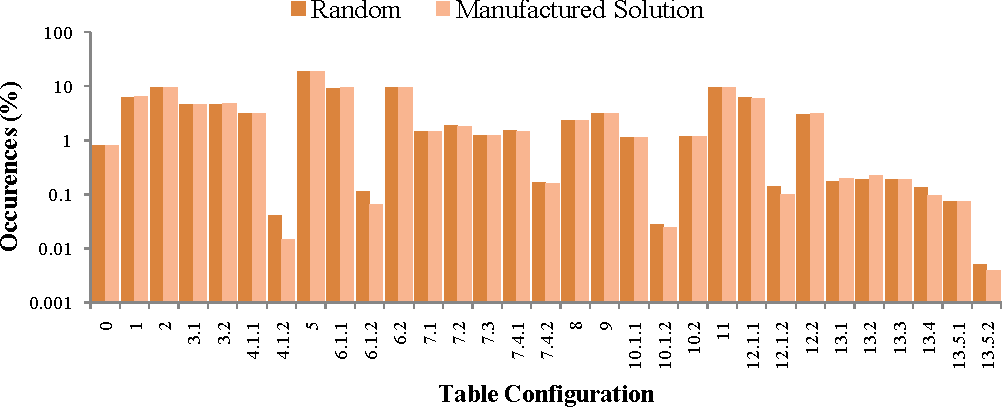
\includegraphics[width=1.0\linewidth,keepaspectratio=true]
{chapter3/figures/random-sampling.pdf}
\caption{The horizontal axis shows the case and subcase numbers for
  each of the 31 Marching Cubes configurations described by Lopes and
  Brodlie~\cite{lopes:tvcg:2003}. The dark bars show the percentage of
  random fields that fit a particular configuration. The light bars
  show the percentage of random fields which fit a particular
  configuration \emph{and} do not violate the assumptions of our
  manufactured solution.  Our manufactured solution hits all possible
  cube configurations.}
\label{fig:cubes-entries}
\end{figure}


% \begin{figure}
% \centering
% \includegraphics[width=0.7\linewidth,keepaspectratio=true]
% {chapter3/figures/mc33-case-00.pdf}
% \caption{An instance of one of the problems uncovered by our framework. From
% left to right: the output from $\proc{MarchingCubes33}$, the expected ouput
% \cite{Lewiner:2003} and the level-set beign extrated. A code mistake prevented
% the extraction of the right configuration.}
% \label{fig:mc33-problem}
% \end{figure}


Table \ref{tbl:verification-ds-stm} shows statistics for all 
implementations. For 
\mclewiner, the tests revealed a problem with configuration 4, 6, and 13 of
the table (ambiguous cases). Figure \ref{fig:problem-mclewiner} shows the
obtained and expected tiles for a cube. 
Contacting the author,
we found that one of the mismatches was due
to a mistake when coding configuration 13 of the MC table. A
non-obvious algorithm detail that is not
discussed in either Chernyaev's or Lewiner's work is the problem of orientation in
some of the cube configurations~\cite{Lewiner:2010:PC}. The case 13.5.2 shown in Figure
\ref{fig:problem-mclewiner} (right) is an example of one such configuration, where
an additional criterion is required to decide the tunnel orientation that is
lacking in the original implementation of \mclewiner. This problem was easily
detected by our framework, because the orientation changes the mesh
invariants, and a mismatch occurs.

\deliso\ presented a high percentage of $\beta_0$ mismatches due to the
mechanism used for tracking connected components. It uses ray-surface intersection to
sample a few points over each connected component of the isosurface before extracting it.
The number of rays is a user-controlled parameter and its initial position
and direction are randomly assigned. \deliso\ is likely to extract the biggest
connected component and, occasionally, it misses small components. It is
important to say that
the ray-sample based scheme tends to work fine in practical applications where
small
surfaces are not present. The invariant mismatches for $\beta_1$ and $\beta_2$
are computed only
if no consistency mismatch happens.

For \mcsimpleflow, we applied the verification
framework systematically during its implementation/development. Obviously, many
bugs were uncovered and fixed over the course of its development. 
%Noticie that this amount of tests is feasable only  using an
%automatic pipeline.
Since we are randomizing the piecewise trilinear field, we are
likely to cover all possible Marching Cubes entries and also different
cube combinations. As verification tests have been applied since the very beginning,
all detectable bugs were removed, resulting in no mismatches. 
The downside of \mcsimpleflow, though, is that typical bad quality
triangles appearing in Marching Cubes become even worse in
\mcsimpleflow,
because cubes of different sizes are glued together. 
\mcsimpleflow\ geometrical
convergence is presented in the supplementary material
\cite{scheidegger:techreport:2010}.

% We finish this section remebering that all three codes \mclewiner, \deliso\
% and \mcsimpleflow\ are still under development and constantly improving. 

\begin{figure}[t]
\centering
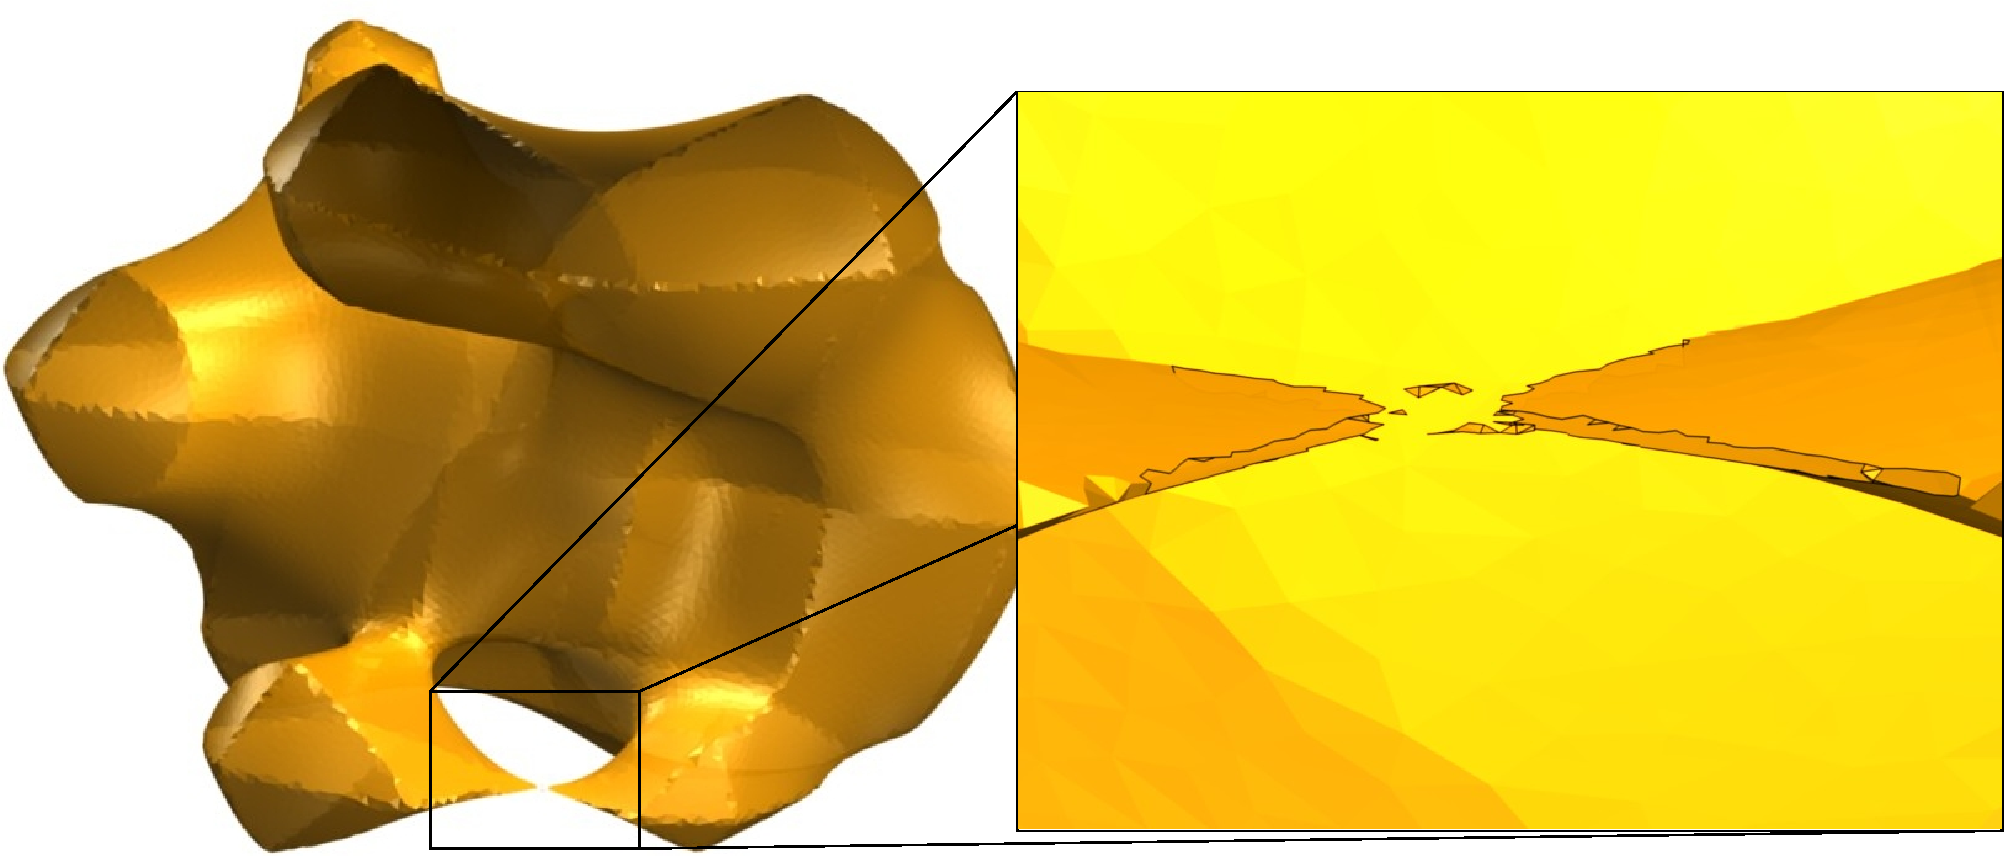
\includegraphics[width=0.33\linewidth,keepaspectratio=true]
{chapter3/figures/deliso-case-00.pdf}
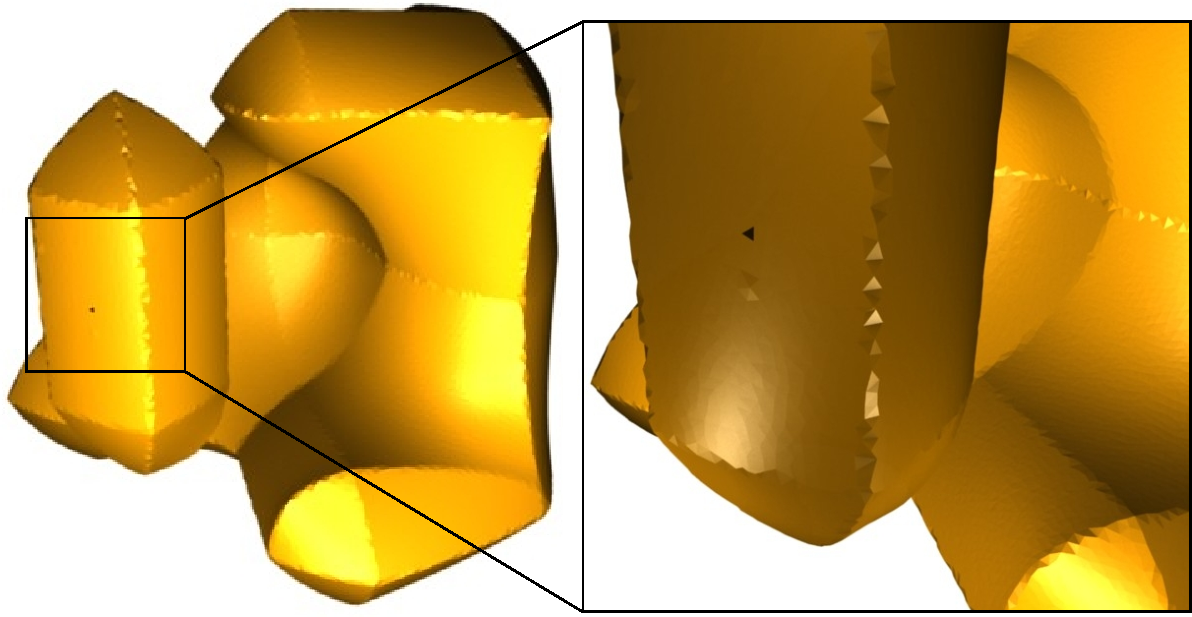
\includegraphics[width=0.3\linewidth,keepaspectratio=true]
{chapter3/figures/deliso-case-02.pdf}
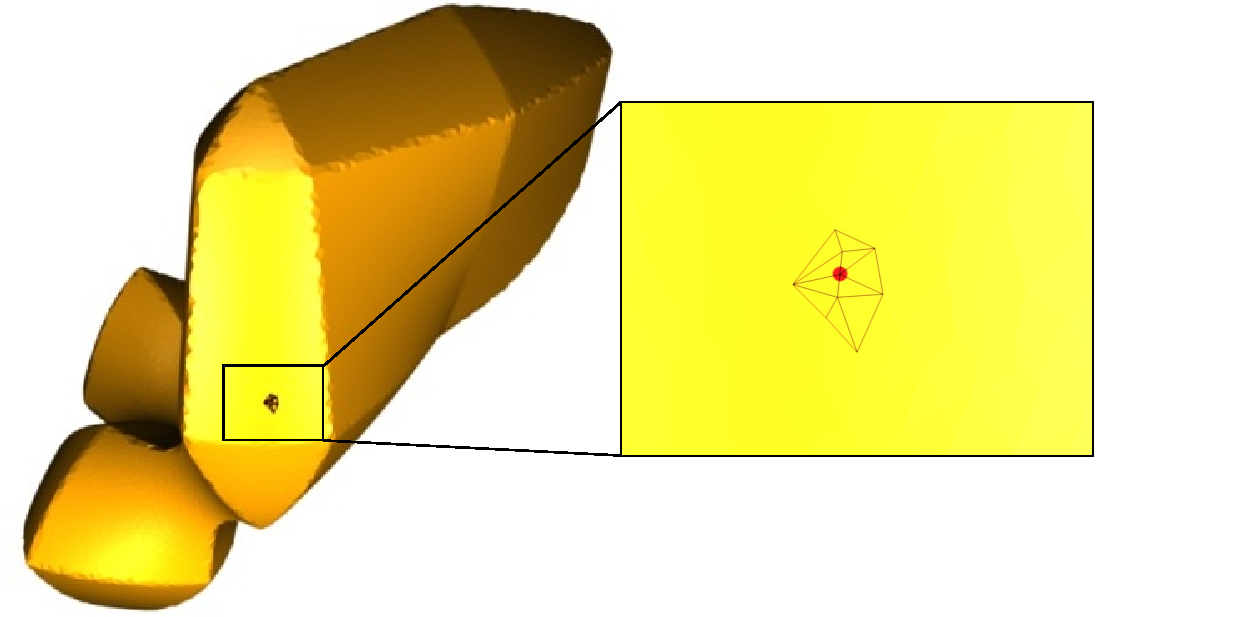
\includegraphics[width=0.29\linewidth,keepaspectratio=true]
{chapter3/figures/deliso-case-03.pdf}
\caption{\deliso\ mismatch example. From left to right: holes in $C^0$
  regions; single missing triangle in a smooth region; duplicated
  vertex (the mesh around the duplicated vertex is shown). These
  behavior induce topology mismatches between the generated mesh and
  the expected topology.}
\label{fig:pproblem-deliso}
\end{figure}

\begin{figure}[t]
\centering
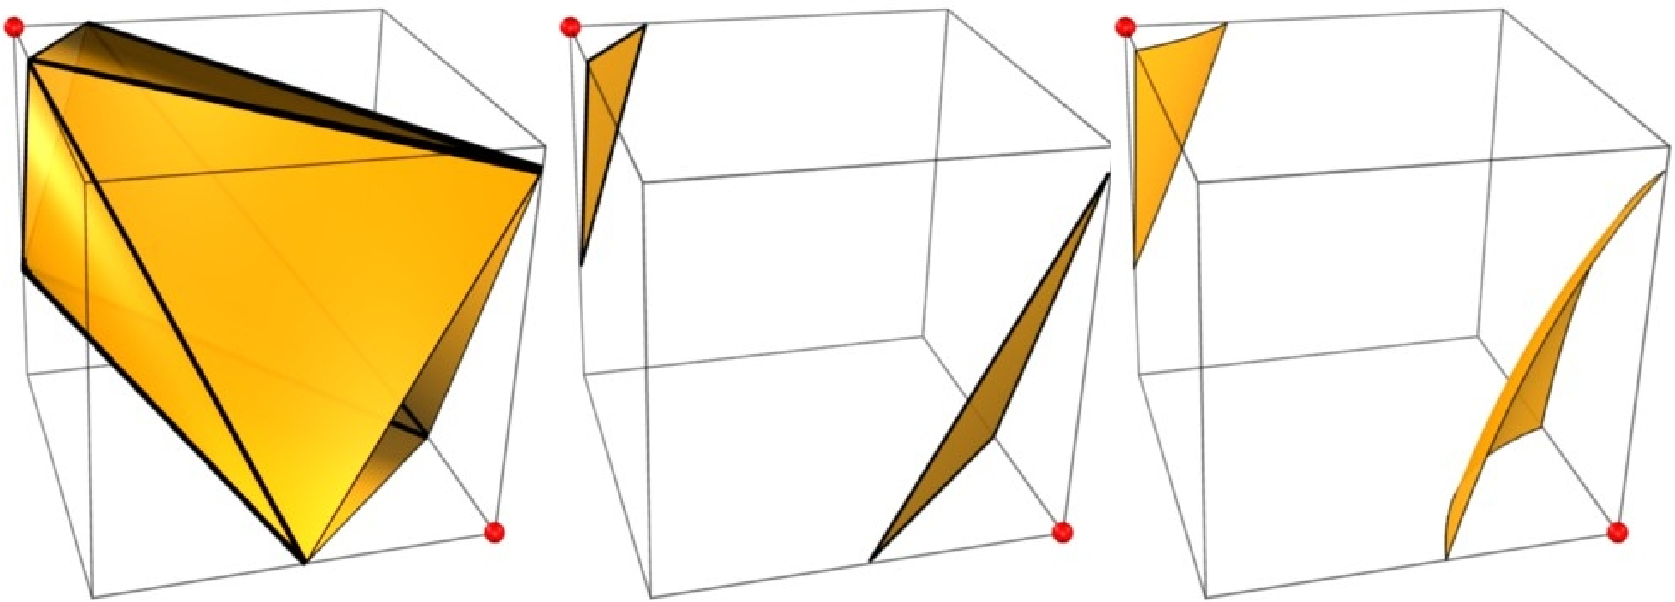
\includegraphics[width=0.3\linewidth,keepaspectratio=true]
{chapter3/figures/mc33-case-02.pdf} ~~~~
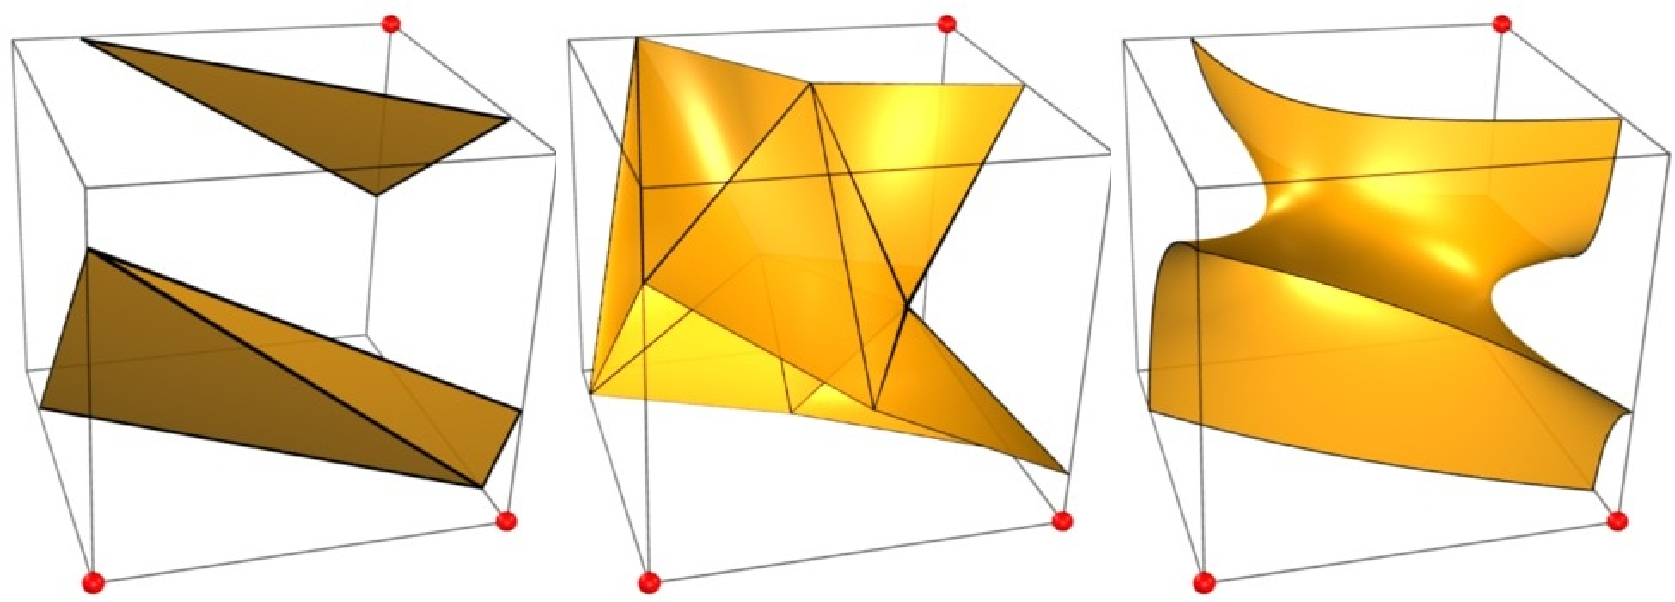
\includegraphics[width=0.3\linewidth,keepaspectratio=true]
{chapter3/figures/mc33-case-01.pdf} ~~~~
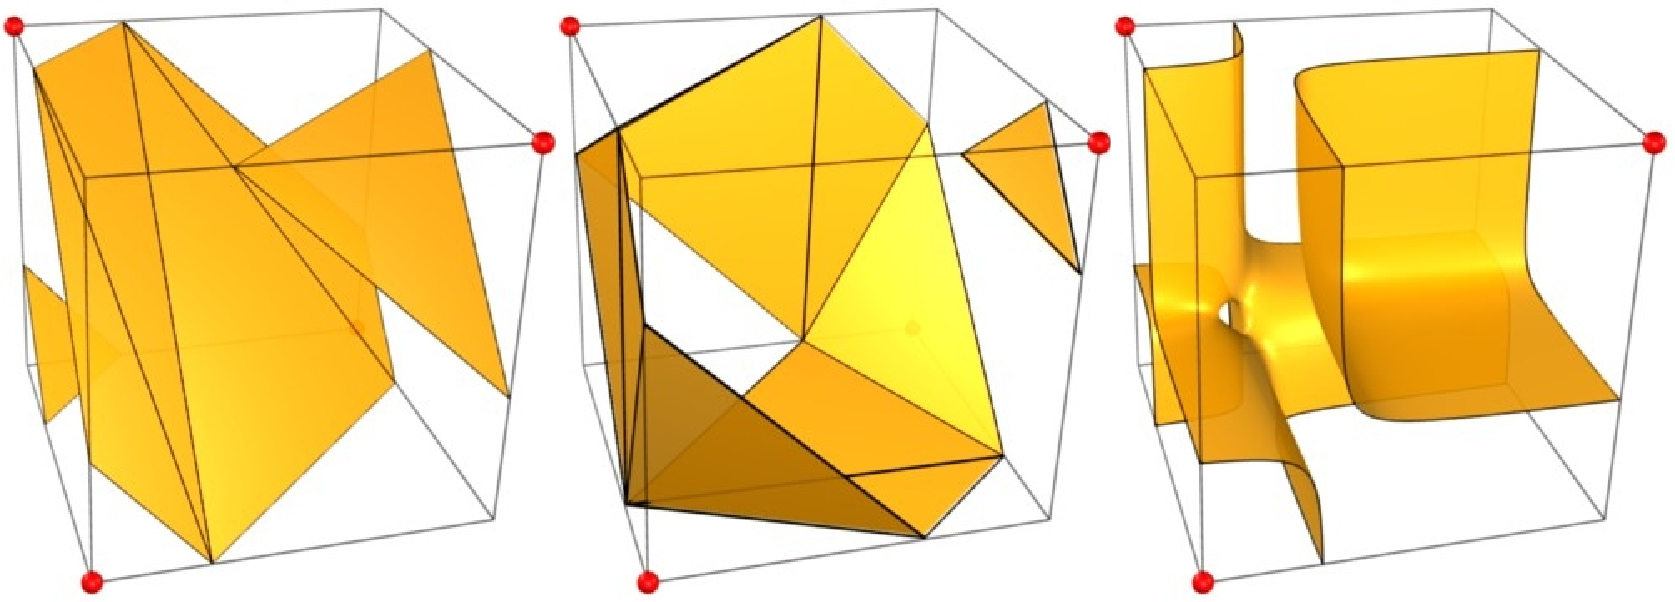
\includegraphics[width=0.3\linewidth,keepaspectratio=true]
{chapter3/figures/mc33-case-00.pdf} 
\caption{\mclewiner\ mismatch example. From left to right: problem in
  the case 4.1.2, 6.1.2, and 13.5.2 of marching cube table (all are
  ambiguous). Each group of three pictures shows the obtained,
  expected, and implicit surfaces. Our verification procedure can
  detect the topological differences between the obtained and expected
  topologies, even for ambiguous cases.}
\label{fig:problem-mclewiner}
\end{figure}


\begin{figure}[t]
\centering
\subfigure[\snapmc\ (0.3)]{
\label{fig:inconsistencies:snapmc}
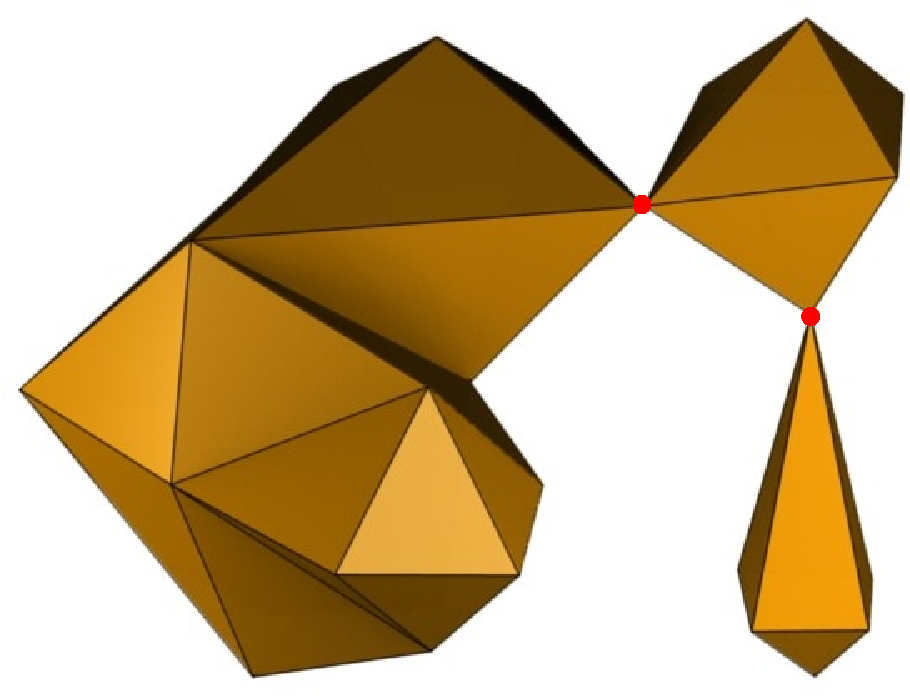
\includegraphics[width=0.20\linewidth,keepaspectratio=true]
{chapter3/figures/snapmc_00.pdf}} ~~~~~~~~
\subfigure[\matlab]{
\label{fig:inconsistencies:matlab}
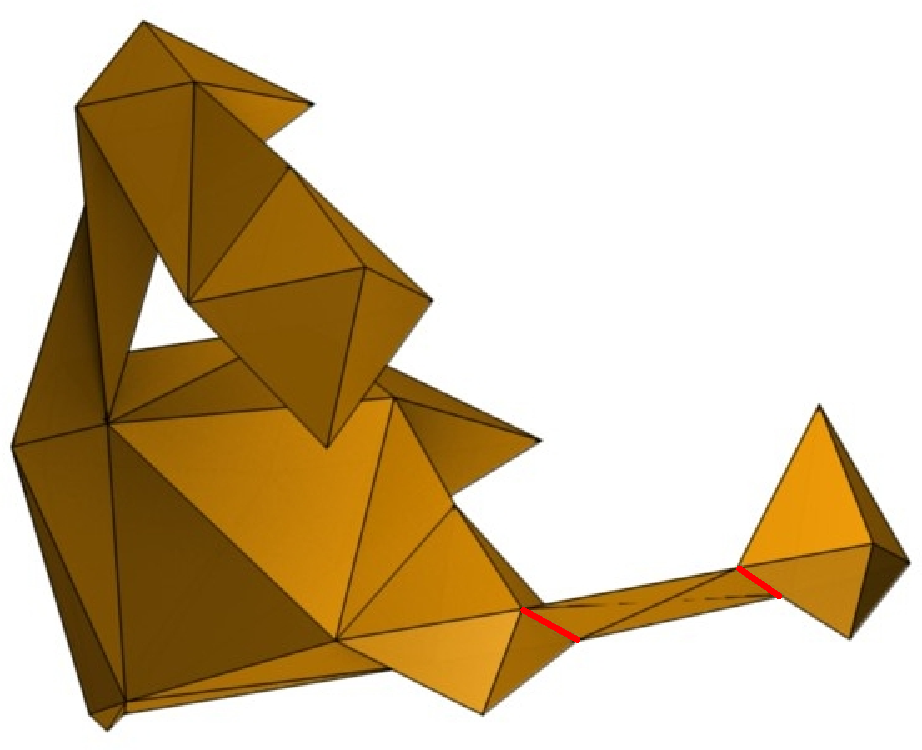
\includegraphics[width=0.20\linewidth,keepaspectratio=true]
{chapter3/figures/matlab_00.pdf}} ~~~~~~~~
\subfigure[\mcsimpleflow]{
\label{fig:problem-mcsimpleflow}
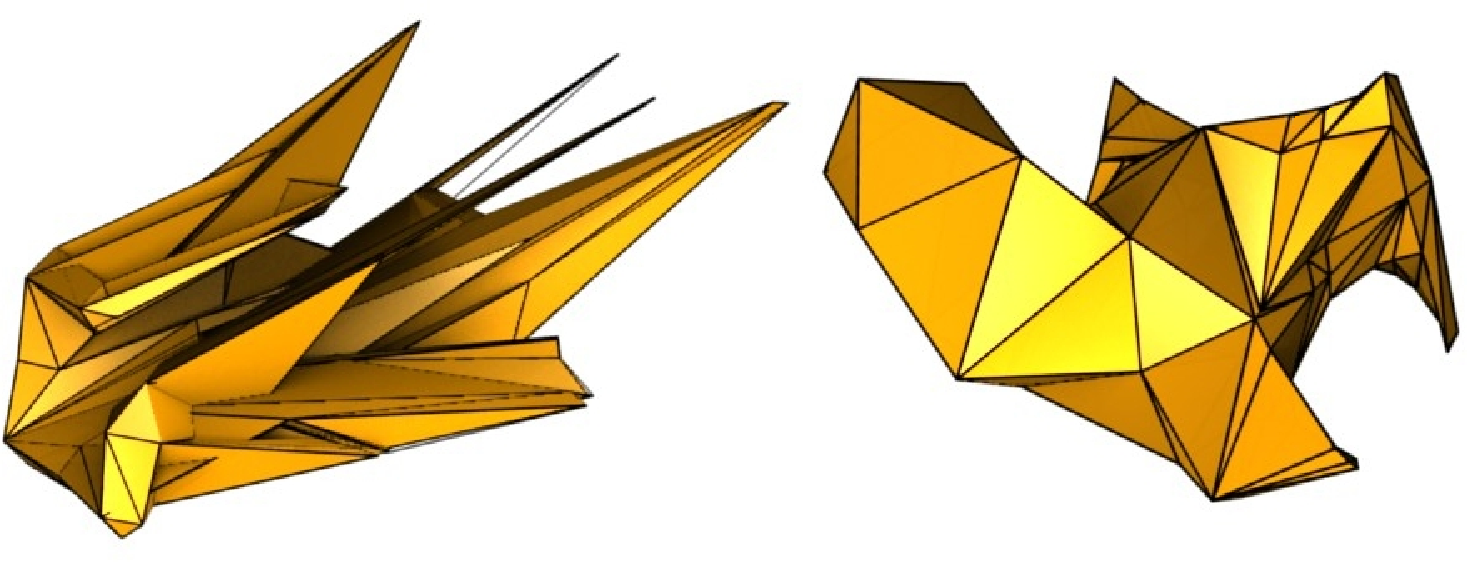
\includegraphics[width=0.37\linewidth,keepaspectratio=true]
{chapter3/figures/our_mc.pdf}}
\caption{Mismatches in topology and geometry. (a) \snapmc\ generates
  non-manifold surfaces due to the snap process. (b)
  \matlab\ generates some edges (red) that are shared by more than two
  face. (c) \mcsimpleflow before (left) and after (right) fixing a bug
  that causes the code to produce the expected topology, but the wrong
  geometry.}
\label{fig:inconsistencies}
\end{figure}


\section{Discussion and Limitations}
\label{sec:discussion}

\subsection{Quality of manufactured solutions}
In any use of MMS, one very important question is that of the quality
of the manufactured solutions, since it reflects directly on the
quality of the verification process. Using random solutions, for which
we compute the necessary invariants, naturally seems to yield good
results. However, our random solutions will almost always have
nonidentical values. This raises the issue of detecting and handling
degenerate inputs, such as the ones arising from quantization. We
note that most implementations use techniques such as Simulation of
Simplicity~\cite{Edelsbrunner:1990:SOS} (for example, by arbitrarily breaking ties using node
ordering) to effectively keep the facade of nondegeneracy. However, we note
that developing manufactured solutions
specifically to stress degeneracies is desirable when using
verification tools during development. We decided against this since
different implementations might employ different strategies to handle
degeneracies and our goal was to keep the presentation sufficiently
uniform.

\begin{table}[b]
\caption{Rate of invariant mismatches using the PL manifold property, digital
surfaces, and stratified Morse theory for $1000$ randomly generated
scalar fields (the lower the rate the better).
The invariants $\beta_1$ and $\beta_2$ are computed only if the output mesh is a
2-manifold without boundary. \emph{We run correctness tests in all algorithms for
completeness and to test tightness of the theory: algorithms that are not
topology-preserving should fail these tests}. 
The high number of \deliso, \snapmc, and \matlab\ mismatches are explained in
Section \ref{sec:consistency}. 
$^1$ indicates zero snap parameter and $^2$ indicates snap value of
0.3.}
\begin{center}
\begin{tabular}{l@{}cccccc}
   & Consistency (\%) &\multicolumn{5}{c}{Correctness (\%)} \\
\hline
    &\multirow{2}{*}{Disk} &\multicolumn{4}{c}{Digital Surfaces} &
SMT\\
              &        &$\beta_0$ & $\beta_1 $ & $\beta_2 $ & $\chi$ & $\chi$ \\
\hline
\afront       & ~$0.0$  & $35.9$  & $22.8$ & $35.9$ & $47.5$ & ~$25.5$
\\
\Matlab       & $19.7$  & $32.2$  & $18.9$ & $20.5$ & $49.3$ & ~$70.3$
\\
\vtk          & ~$0.0$  & $27.6$  & $23.2$ & $27.6$ & $43.5$ & ~$70.7$
\\
\hline
\macet        & ~$0.0$  & $54.3$  & $20.9$ & $54.3$ & $64.0$ & $100.0$
\\
\snapmc$^1$   & ~$0.0$  & $45.0$  & $25.4$ & $45.0$ & $57.3$ & ~$72.0$
\\
\snapmc$^2$   & $53.7$  & $41.6$  & $17.3$ & $23.1$ & $87.1$ & ~$74.0$
\\
\hline
\mclewiner    & ~$0.0$  & ~$2.4 $ & ~$1.1$ & ~$2.4$ & ~$3.4$ & ~~$5.4$ 
\\
\deliso       & $19.1$  & $24.4$  & ~$0.1$ & $20.0$ & $37.2$ & ~$33.2$ 
\\
\mcsimpleflow & ~$0.0$  & ~$0.0$  & ~$0.0$ & ~$0.0$ & ~$0.0$ & ~~$0.0$ 
\\
\hline
\end{tabular}
\label{tbl:verification-ds-stm}
\end{center}
\end{table}


\subsection{Topology and Geometry}
This work extends the work by Etiene \emph{et al.}~\cite{etiene:tvcg:2009} toward
including topology in the loop of verification for isosurface techniques. 
The machinery presented herein combined with the methodology for verifying
geometry comprises a solid battery of tests able to stress most of the existing 
isosurface extraction codes. 

To illustrate this, we also submitted \mclewiner\ and \mcsimpleflow\ techniques 
to the geometrical test proposed by Etiene, as these codes have not been 
geometrically verified. While \mclewiner\ has geometrical
behavior in agreement with Etiene's approach, the results presented in Section~\ref{sec:results} 
show it does not pass the topological tests. 
%our framework revealed a code mistake. 
On the other hand, after ensuring that 
\mcsimpleflow\ was successful regarding topological tests, 
we submitted it to the geometrical analysis, which revealed problems.
Figure \ref{fig:problem-mcsimpleflow} shows an
example of an output generated in the early stages of development of \mcsimpleflow\ before (left) and after
(right) fixing the bug. The topology matches the expected one (a
topological sphere); nevertheless, the geometry does not converge. 


% \paragraph*{Interpreting behavior}
% We have talked to the authors of two of the techniques under verification to
% understand the behavior shown in Table \ref{tbl:verification-ds-stm}. As
% explained earlier, \mclewiner\ had a code mistake that prevent it from
% generate
% the right topology for configuration 13.5.2 of Marching Cubes table. Even
% after
% fixing it, there were still some mismatches that need to be explained which
% motivates the verification cycle. 
% \paragraph*{Topology Consistency vs. Correctness}

\subsection{SMT vs. DT}
The verification approach using digital surfaces generates detailed
information about the expected topology because it provides $\beta_0$, $\beta_1$, and $\beta_2$. 
However, verifying isosurfaces with boundaries would require
additional theoretical results, as the theory supporting our verification
algorithm is only valid for surfaces without boundary.
%The current framework does not deal with surfaces touching the
%boundary of the domain although it can be extended to account for it. 
In contrast, the verification methodology using stratified Morse theory can handle
surfaces with boundary. However, SMT only provides information 
about the Euler characteristic, making it harder to determine when the topological verification process fails.
%Since many application requires extraction of isosurfaces with boundaries, it is
%also important they are computed correctly. 
Another issue with SMT is that if a code incorrectly introduces topological features so as
to preserve $\chi$, then no failure will be detected. For example, suppose the surface to
be reconstructed is a torus, but the code produces a torus plus three triangles,
each one sharing two vertices with the other triangles but not an edge. In this case, 
torus plus three ``cycling'' triangles also has $\chi = 0$, exactly the Euler characteristic of the single torus.
In that case, notice that the digital surface-based test would be able to
detect the spurious three triangles by comparing $\beta_0$.
Despite being less sensitive in theory, 
SMT-based verification revealed similar problems as the digital topology tests have. 
We believe this effectiveness comes in part from 
the randomized nature of our tests.

\subsection{Implementation of SMT and DT}
Verification tools should be as simple as possible while still
revealing unexpected behavior. The pipeline for geometric
convergence is straightforward and thus much less error-prone. This is
mostly because
Etiene \emph{et al.}'s approach uses analytical manufactured solutions to provide
information about function value, gradients, area, and curvature. In topology,
on the other hand, we can manufacture only simple analytical solutions (e.g., a
sphere, torus, double-torus, etc.) for which we know topological
invariants. There are no guarantees that these solutions will cover all
cases of a trilinear interpolant inside a cube. For this reason, we
employ a random manufactured solution and must then compute
explicitly the topological invariants.
A point which naturally arises in verification settings is that the verification code is another program. 
How do we verify the verifier?

First, note that the implementation of either verifier is simpler than
the isosurfacing techniques under scrutiny. This reduces the chances
of a bug impacting the original verification.  In addition, we can use
the same strategy to check if the verification tools are implemented
correctly. For SMT, one may compute $\chi$ for an isovalue that is
greater than any other in the grid. In such case, the verification
tool should result in $\chi = 0$. For DT, we can use the fact that
Majority Interpolation always produces a 2-manifold. Fortunately, this
test reduces to check for two invalid cube configurations as described
by Stelldinger \emph{et al.}~\cite{siqueira:2007}. Obviously, there might
remain bugs in the verification code. As we have stated before, a
mismatch between the expected invariants and the computed ones
indicates a problem \emph{somewhere} in the pipeline; our experiments
are empirical evidence of the technique's effectiveness in detecting
implementation problems.

Another concern is the performance of the verification tools. In our
experiments, the invariant computation via SMT and DS is faster than
any isosurface extraction presented in this work, for most of the
random grids. In some scenarios, DS might experience a slowdown
because it refines the grid in order to eliminate ambiguous cubes (the
maximum number of refinement is set to 4). Thus, both SMT and DS (after
grid refinement) need to perform a constant number of operations
for each grid cube to determine the digital surface (DS) or critical
points (SMT).  In this particular context, we highlight the recent
developments on certifying algorithms, which produce both the
output and an \emph{efficiently checkable certificate of
  correctness}\cite{McConnell:2010:CA}.


\subsection{Contour Trees}
Contour trees \cite{Hamish03} are powerful structures to describe the
evolution of level-sets of simply connected domains. It normally
assumes a simplicial complex as input, but there are extensions to
handle regular grids\cite{Pascucci03}. Contour trees naturally provide
$\beta_0$, and they can be extended to report $\beta_1$ and
$\beta_2$. Hence, for any isovalue, we have information about all
Betti numbers, even for surfaces with boundaries.  This fact renders
contour trees a good candidate for verification purposes. In fact, if an
implementation is available, we encourage its use so as to increase
confidence in the algorithm's behavior.  However, the implementation of
a contour tree is more complicated than the techniques presented here.
For regular-grids, a divide-and-conquer approach can be used along
with oracles representing the split and join trees in the deepest
level of the recursion, which is non-trivial. Also, implementing the
merging of the two trees to obtain the final contour tree is still
involving and error-prone.  Our approach, on the other
hand, is based on regular grid refinement and voxel selection for the DT
method and critical point computation and classification for the SMT
method.  There are other tools, including contour trees, that could be
used to assess topology correctness of isosurface extraction
algorithms, and an interesting experiment would be to compare the
number of mismatches found by each of these tools.  Nevertheless, in
this work, we have focused on the approaches using SMT and DT because
of their simplicity and effectiveness in finding code
mistakes in publicly available implementations.  We believe that the
simpler methodologies we have presented here are more likely to be
adopted during development of visualization isosurfacing tools.

\subsection{Topology of the underlying object}
In this work, we are interested in how to effectively verify
topological properties of codes which employ trilinear
interpolation. In particular, this means that our verification tools
will work for implementations other than marching methods (for
example, DelIso is based on Delaunay refinement).
%
Nevertheless, in practice, the original scalar field will not be
trilinear, and algorithms which assume a trilinearly interpolated
scalar field might not provide any topological guarantee regarding the
reconstructed object.
%scientists may be interested in the topology of the \emph{original
%object} instead of a trilinear interpolant. 
Consider, for example, a piecewise linear curve $\gamma$ built by
walking through diagonals of adjacent cubes $c_i \in \mathcal{G}$ and
define the distance field $d(x) = \min\{||x - x'||\, \text{such
  that}\ x'\in\gamma\}$. The isosurface $d(x) = \alpha$ for any
$\alpha > 0$ is a single tube around $\gamma$.  However, none of the
implementations tested could successfully reproduce the tubular
structure for all $\alpha > 0$. This is not particularly surprising,
since the trilinear interpolation from samples of $d$ is quite
different from the $d$.
\begin{figure}[b]
\centering
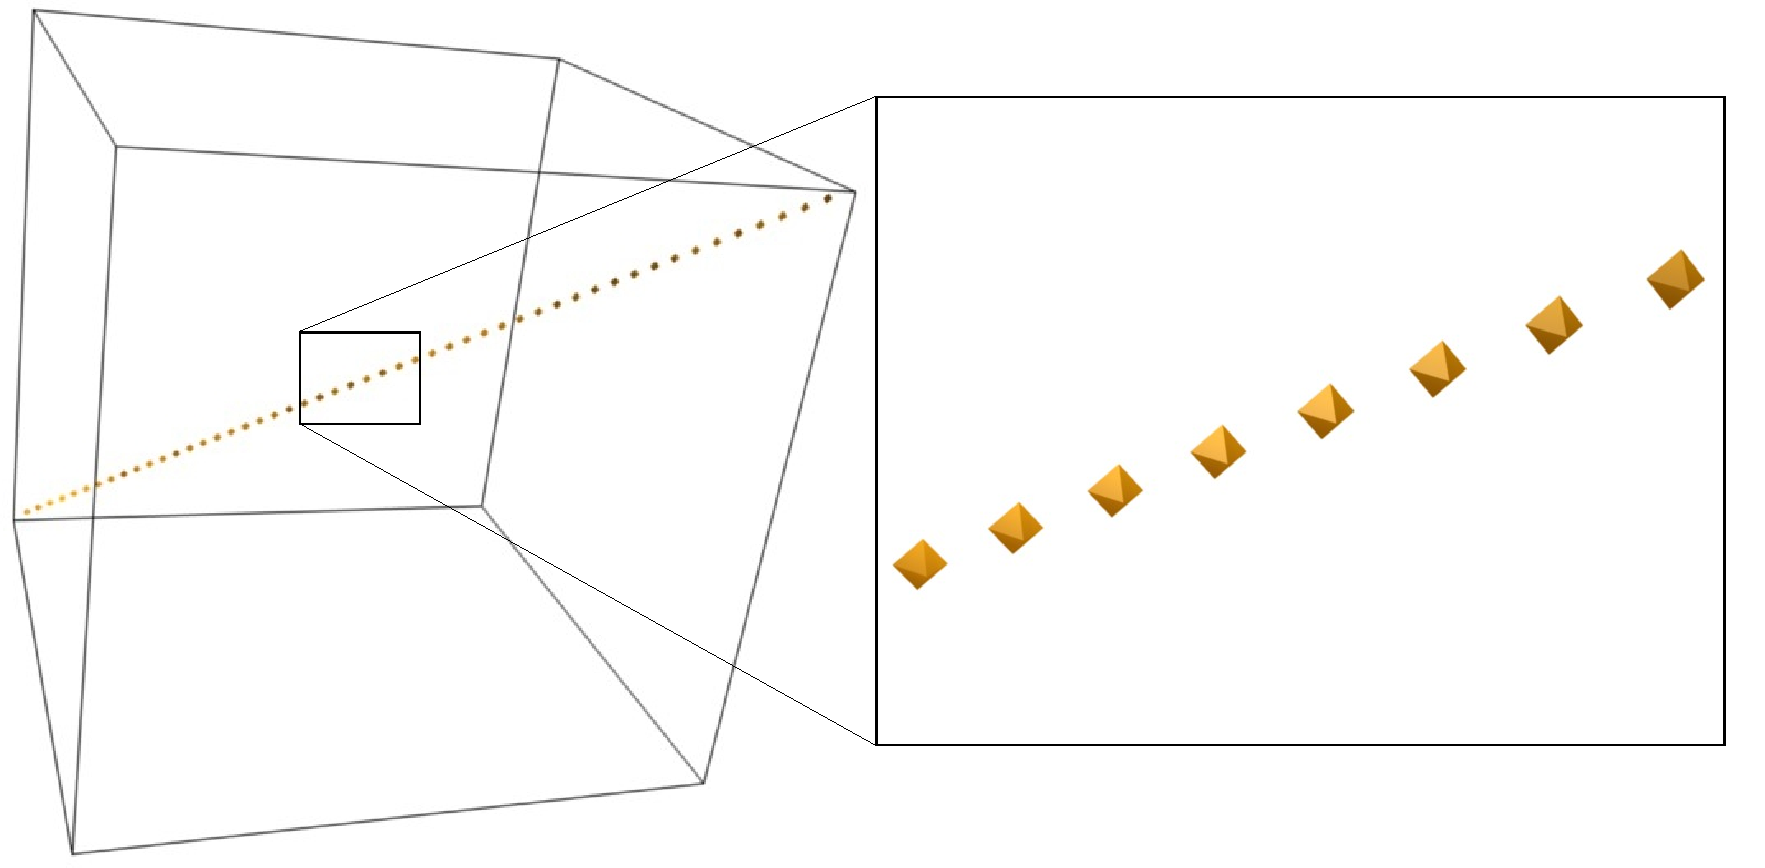
\includegraphics[width=0.5\linewidth]{chapter3/figures/distance-field.pdf}
\caption{\label{fig:chap4:vtk} Isosurface extracted with VTK Marching Cubes}
\end{figure}
Figure \ref{fig:chap4:vtk} on the right shows a typical output produced by VTK
Marching Cubes for the distance field $d = \alpha$. Notice, however,
that this is not only an issue of sampling rate because if the tube
keeps going through the diagonals of cubic cells, VTK will not be able
reproduce $d = \alpha$ yet.  Also recall that some structures cannot
even be reproduced by trilinear interpolants, as when
$\gamma$ crosses diagonals of two parallel faces of a cubic cell, as
described in \cite{Chernyaev95marchingcubes, Pascucci03}.  The aspects
above are not errors in the codes but reflect software design choices
that should be clearly expressed to users of those visualization
techniques.

%Other interpolants could be used to reconstructu guiding the meshing
%template in each cube considering that this is an issue related to
%the disambiguation scheme employed and not necessarily a code
%mistake.  In the scenario described above, the isovalue can be
%changed slightly or the disambiguation scheme could be altered in
%order to reproduce the tubes correctly but some curves crossing
%cannot even be reproduced by trilinear interpolant Any interpolant
%can be used to approximate the topology of the original
%object. However, there are only a handful of cases were one can
%guarantee that the extracted surface is homeomeorphic to the
%underlying object.

\subsection{Limitations}
The theoretical guarantees supporting our manufactured solution
rely on the trilinear interpolant.  
If an interpolant other than trilinear is employed, then new results ensuring
homeomorphism (Theorem 4.1) should be derived. 
The basic infrastructure we have described here, however,
should be appropriate as a starting point for the process.


\section{Conclusion}

In this chapter, we extended the framework presented in the previous chapter
by including topology into the verification
cycle.  We used machinery from digital topology and stratified Morse
theory to derive two verification tools that are simple and yet
capable of finding unexpected behavior and coding mistakes.
%
We argue that researchers and developers should consider adopting
verification as an integral part of the investigation and development
of scientific visualization techniques.  Topological properties are as
important as geometric ones, and they deserve the same amount of
attention. It is telling that the only algorithm that passed all
verification tests proposed here is the one that used
the verification procedures \emph{during} its development. We believe
this happened because topological properties are particularly subtle
and require an unusually large amount of care.

%% if specified like this the section will be ommitted in review mode
%\section*{Acknowledgments}
%We thank Thomas Lewiner and Joshua Levine for
%  help with \mclewiner\ and \deliso\ codes respectively.
%This work was supported in part by grants from
%%  the National Science Foundation
%  NSF
% (grants IIS-0905385, IIS-0844546,
%  ATM-0835821, CNS-0751152, OCE-0424602, CNS-0514485, IIS-0513692,
%  CNS-0524096, CCF-0401498, OISE-0405402, CCF-0528201, CNS-0551724,
%  CMMI 1053077, IIP 0810023, CCF 0429477),
%  DOE,
%%  the Department of Energy, 
%  IBM Faculty Awards and PhD Fellowship, the
%  US ARO % Army Research Office
%  under grant W911NF0810517, ExxonMobil, and
%  Fapesp-Brazil (\#2008/03349-6).

